


\chapter{Sampling}


\section{References}

This chapter is mainly taken from \cite{signal_processing_Lathi}.

\section{Introduction to Sampling and Reconstruction}

Sampling is a common operation in signal processing, since our computers and hardware we use process \tbi{discrete sample}. An example is shown in \autoref{fig:Sampling:Sampling_Example}.


\begin{figure}[h]
\centering
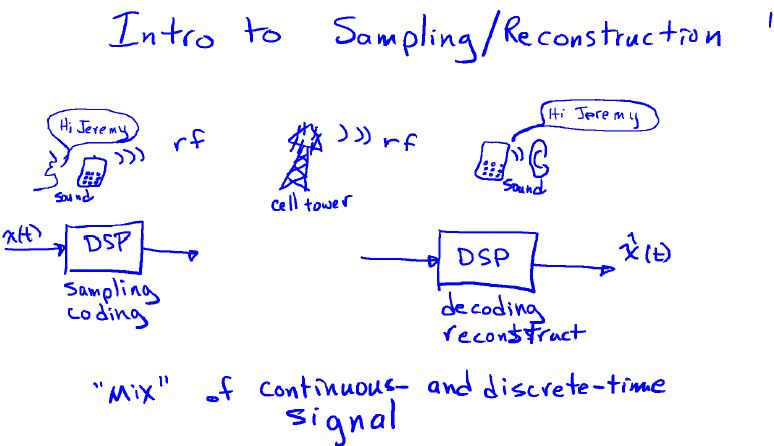
\includegraphics[width = 0.7\textwidth, frame]{Figures/Sampling/Sampling_Example}
\caption{Example of Sampling: digital transmission}
\label{fig:Sampling:Sampling_Example}
\end{figure}

\begin{itemize}

\item We have some sound denoted by $x(t)$

\item Inside the phone, there is some DSP chip which do the sampling and the coding process

\item Then some hardware to modulate the signal to transform it into RF signal for transmission

\item At the receiver, the signal is demodulated back to the base band status

\item Then a decoding and reconstruction process is done to reconstruct the original signal $x(t)$.

\end{itemize}

The goal is that we hope that $\hat{x}(t) \, \approx \, x(t)$.\\

We will use the Fourier transform to analyze the effect of sampling and tackle the problem of reconstruction, and also we ask several question to build an efficient system which can do this reconstruction:

\begin{itemize}
\item How fast do we need to sample ?

\item How to reconstruct ?
\end{itemize}


\section{Sampling Continuous Time Signals}
\label{Sec:Sampling:Sampling_Continuous_Time_Signals}



\subsection{Impulse Sampling Analysis using Fourier Transform}

To do the mathematical derivation later.

\subsection{Intuition and Interpretation}

\begin{figure}[h]
\centering
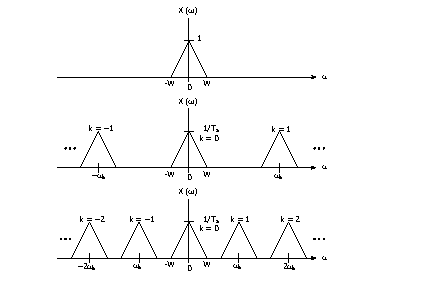
\includegraphics[width = 0.7\textwidth, frame]{Figures/Sampling/impulse_sampling_spectrum_1}
\caption{Sampling Higher then the Nyquite Rate}
\label{fig:Sampling:impulse_sampling_spectrum_1}
\end{figure}

\begin{itemize}
\item When sampling higher then the Nyquist rate, we could still distinguish the original version of the spectrum, which is in the middle
\end{itemize}


\newpage
Let's try now to decrease the sampling rate ($\omega_s$ decrease) as shown in \autoref{fig:Sampling:impulse_sampling_spectrum_2}.


\begin{figure}[h]
\centering
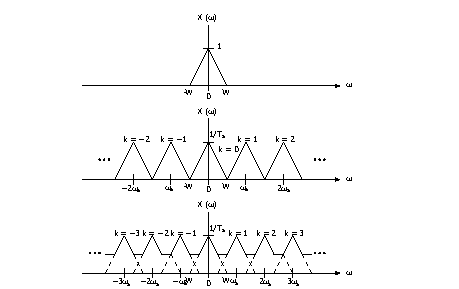
\includegraphics[width = 0.7\textwidth, frame]{Figures/Sampling/impulse_sampling_spectrum_2}
\caption{Decreasing the Nyquist Rate: Aliasing Result}
\label{fig:Sampling:impulse_sampling_spectrum_2}
\end{figure}

\begin{itemize}

\item When decreasing the sampling rate $\omega_s$, the shifted spectrum get close to each other

	\begin{itemize}
	\item In the $\mathrm{2}^\mathrm{nd}$ row of \autoref{fig:Sampling:impulse_sampling_spectrum_2}, we are sampling exactly at the Nyquist rate
	
	\item No gap between the original spectrum and the shifted version
	\end{itemize}


\item When sampling rate $\omega_s$ less then the \tbi{Nyquist rate}, the shifted versions have collide with the original spectrum 

	\begin{itemize}
	\item The only thing we can see is the blue solid line
	
	\item We could not retrieve the original spectrum as before now.
	\end{itemize}

\end{itemize}



\subsection{Example: Sampling a Cosine}

Let's take the signal $x(t) \, = \, \text{cos}\left( \pi t \right)$, and sample this signal at different sampling rate $\omega_s$ and study the effect for different values of $\omega_s$.

\begin{figure}[h]
\centering
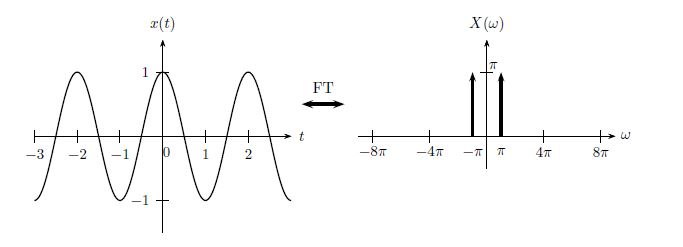
\includegraphics[width = 0.7\textwidth, frame]{Figures/Sampling/Sampling_cosine}
\caption{Example of Sampling a cos: period $\, = \, 2$ s}
\label{fig:Sampling:Sampling_cosine}
\end{figure}


\newpage
First case we take $\omega_s \, = \, 8 \pi \rightarrow \, T_s \, = \, \displaystyle\frac{1}{4}$s. Case is shown in \autoref{fig:Sampling:Sampling_cosine_2}.

 
\begin{figure}[h]
\centering
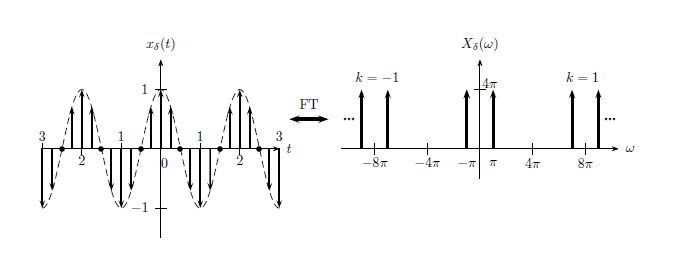
\includegraphics[width = 0.7\textwidth, frame]{Figures/Sampling/Sampling_cosine_2}
\caption{$\omega_s \, = \, 8 \pi \, ; \, T_s \, = \, \displaystyle\frac{1}{4}$ s}
\label{fig:Sampling:Sampling_cosine_2}
\end{figure}

	\begin{itemize}
	\item The shifted spectrum are repeated at multiple of $\omega_s$
	
	\item Don't forget that we have the scale factor $\displaystyle\frac{1}{T_s} \, = \, 4$
	\end{itemize}
	
Case 2 shown in \autoref{fig:Sampling:Sampling_cosine_3}: we decrease $\omega_s$ to become $2\pi \rightarrow \, T_s \, = \, 1$s. So we take less samples per second.

\begin{figure}[h]
\centering
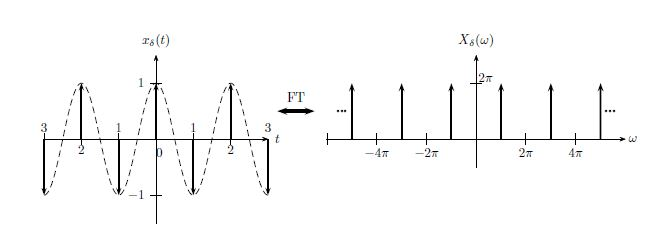
\includegraphics[width = 0.7\textwidth, frame]{Figures/Sampling/Sampling_cosine_3}
\caption{Exactly Sampling at Nyquist rate ; $\omega_s \, = \, 2 \pi \, ; \, T_s \, = \, 1$ s}
\label{fig:Sampling:Sampling_cosine_3}
\end{figure}

\begin{itemize}
\item The case shown in \autoref{fig:Sampling:Sampling_cosine_3}: we are sampling \tbi{exactly at the Nyquist rate} where $\omega_s \, = \, 2 W$ and $W \, = \, \pi$.

\item We are still able to see the original spectrum located at $\pi$ and $-\pi$

\item However notice that at the scaling factor: it is true that $\displaystyle\frac{1}{T_s} \, = \, 1$, but we have $2 \pi$

	\begin{itemize}
	
	\item This is because when we shift the original spectrum at multiple of $\omega_s$, the dirac shifted land on top of the original dirac , and added together	
	
	\end{itemize}

\end{itemize}

\newpage
Last case shown in \autoref{fig:Sampling:Sampling_cosine_4} is we sample below Nyquist rate and aliasing effect occur also.


\begin{figure}[h]
\centering
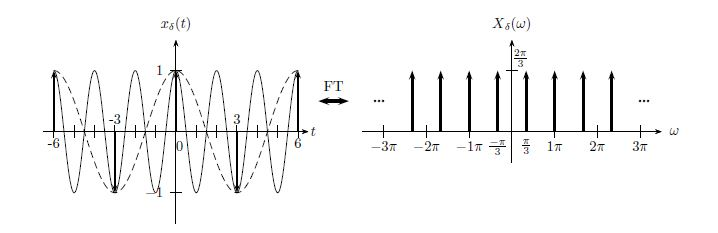
\includegraphics[width = 0.7\textwidth, frame]{Figures/Sampling/Sampling_cosine_4}
\caption{Sampling below Nyquist rate ; $\omega_s \, = \displaystyle\frac{2 \pi}{3} \, ; \, T_s \, = \, 3$ s}
\label{fig:Sampling:Sampling_cosine_4}
\end{figure}


\begin{itemize}

\item Because we are sampling below the Nyquist rate, the reconstructed cosine appear to be a low frequency one

\item This is can be deduced from the frequency spectrum: notice that when the spectrum is shifted at multiple of $\omega_s \, = \, \displaystyle\frac{2 \pi}{3}$, 

	\begin{itemize}
	
	\item the dirac component located at $-\pi$ (this is the original one) is shifted to $\displaystyle\frac{-\pi}{3}$	
	
		\item Same for the dirac component located at $+\pi$ (this is also the original one) is shifted to $\displaystyle\frac{+\pi}{3}$
		
		\item So it seems that the original spectrum is located at $\left[\, \displaystyle\frac{-\pi}{3} \, ; \, \displaystyle\frac{+\pi}{3} \, \right]$
	
	\end{itemize}

\end{itemize}


\subsection{Predicting Aliasing frequency}

We have seen in \autoref{fig:Sampling:Sampling_cosine_4} that when we sample below the Nyquist rate, aliasing occurred and the cos signal has transformed from high frequency $f \, = \, \displaystyle\frac{1}{2}$ Hz to $f_{\text{alias}} \, = \, \displaystyle\frac{1}{3}$ Hz. In this section we try to use some equations in order to predict in advance the aliasing frequency $f_{\text{alias}}$.\\

The equation are:

\begin{equation}
\begin{array}{rcl}
f_{\text{alias}} \, &\leq& \, \displaystyle\frac{Fs}{2} \\
f_{\text{alias}} \, &=& \, \lvert f_{\text{original}} \, - \, m \, f_s  \rvert \quad \text{where } m \, = \, 0 \, ; \, 1 \, ; \, 2 ;\, \cdots
\end{array}
\label{Eq:Sampling:alias_frequency}
\end{equation} 

\newpage
An example is shown in \autoref{fig:Sampling:alias_frequency}.

\begin{figure}[h]
\centering
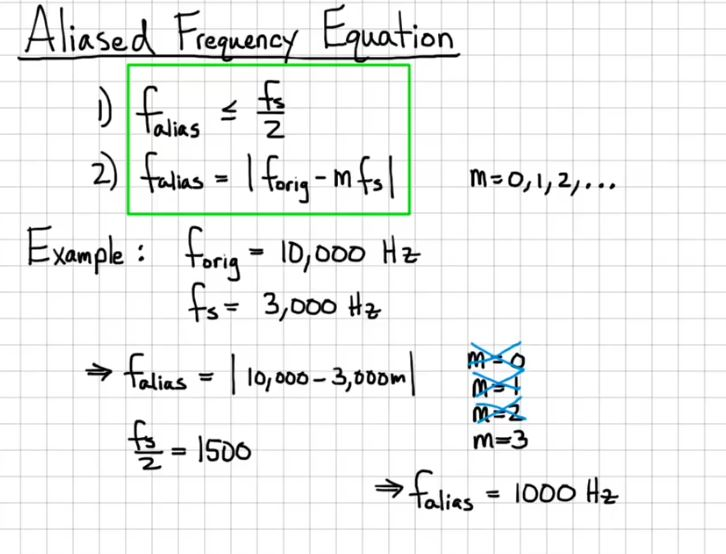
\includegraphics[width = 0.7\textwidth, frame]{Figures/Sampling/alias_frequency}
\caption{Predicting alias frequency}
\label{fig:Sampling:alias_frequency}
\end{figure}

\begin{itemize}

\item We have some signal where $f_{\text{original}} \, = \, 10^4$ Hz

\item We sample the signal with $f_s \, = \, 3000$ Hz

	\begin{itemize}
	\item Clearly, aliasing will occur since we dind't respect the Nyquist condition
	\end{itemize}


\item We keep using \ref{Eq:Sampling:alias_frequency}:

	\begin{itemize}
	
	\item We solve for $m \, = \,0$, we obtain $f_{\text{alias}} \, = \, 10^4$. This $f_{\text{alias}}$ doesn't satisfy the condition $f_{\text{alias}} \, \leq \, \displaystyle\frac{Fs}{2} $, so we keep solving for other value of $m$.
	
	
	\item For $m \, = \, 3$, we get $f_{\text{alias}} \, = \, 10000$ Hz, and this frequency satisfy the condition $f_{\text{alias}} \, = \, 1000 \, \text{Hz} \, \leq \, \displaystyle\frac{Fs}{2} $ 
	
	\end{itemize}

\end{itemize}

So when we sample a signal of $f_{\text{original}} \, = \, 10^4$ Hz with $f_s \, = \, 3000$ Hz, we get an alias frequency of 1000 Hz.


\newpage
\section{Examples}

Consider the analog signal: $x(t) \, = \, 4 \, + \, 2\, \text{cos}\left(\, 150 \pi t \, + \, \displaystyle\frac{\pi}{3} \,\right) \, + \, 4 \, \text{sin}\left(\, 350 \pi t \,\right)$.\\

To be done later.


\section{Other Practical Considerations}

In this section we look to more sophisticated points related to sampling, like the fact that in \tbi{real world signals}, they are always time limited, and the implication of this time limitation on sampling. Also we deals with several \tbi{application to sampling} like pulse modulation,$\cdots$.

\subsection{Time Limited Signals}

The time-bandwidth product also know as \tbi{uncertainty principle} is shown in equation (\ref{Eq:time_band_produc}) 

\begin{equation}
\begin{array}{rcl}
T_d \, &=& \, \left[ \displaystyle\frac{\int\limits_{-\infty}^{+\infty}  t^2 \, |x(t)|^2 \, dt}{\int\limits_{-\infty}^{+\infty} |x(t)|^2 \, dt} \right]^{0.5} \\ \\
B_w \, &=& \, \left[ \displaystyle\frac{\int\limits_{-\infty}^{+\infty}  \omega^2 \, |X(\omega)|^2 \, d\omega}{\int\limits_{-\infty}^{+\infty} X|(\omega)|^2  \, d\omega} \right]^{0.5} \\ \\
T_d \, \times \, B_{\omega} \, &\geq& \, 0.5
\end{array}
\label{Eq:time_band_produc}
\end{equation}

Equation (\ref{Eq:time_band_produc}) says that if we have a \tbi{time limited signal} , the \tbi{frequency content} of the signal will \tbi{extent to infinity}, and hence this will cause a \tbi{problem when doing sampling}. Sampling theorem tell us that we need to sample at the Nyquist rate $F_s$ where $F_s$ is at least 2 times higher than the maximum frequency of the signal. Since the maximum frequency is infinity, we can't sample at infinity, and \tbi{this cause any frequency content above $\displaystyle\frac{F_s}{2}$ to fold with the original spectrum}. 


\newpage
This is illustrated in \autoref{fig:Sampling:Folding}.


\begin{figure}[h]
\centering
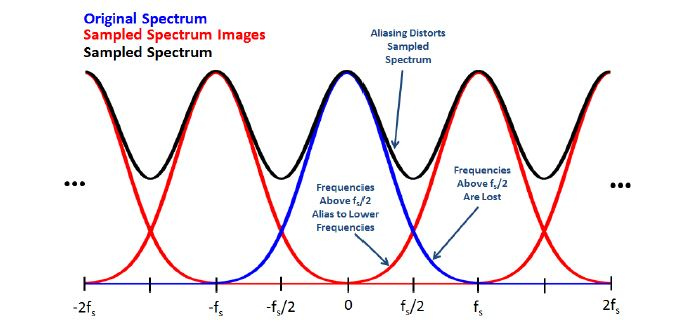
\includegraphics[width = 0.7\textwidth, frame]{Figures/Sampling/Folding}
\caption{Signal Aliasing: frequency at $\displaystyle\frac{F_s}{2} \, + \, f_x$ shows at $\displaystyle\frac{F_s}{2} \, - \, f_x$}
\label{fig:Sampling:Folding}
\end{figure}

\begin{itemize}

\item We have the original theoretical spectrum in blue we wish to recover

\item We know from sampling theorem that due to sampling, the spectrum will get replicated at multiple of $F_s$, and the resultant spectrum will be the summation of all the copies at every point, which give us the black spectrum.

\end{itemize}

Now when we wish to recover the spectrum (the blue one in  \autoref{fig:Sampling:Folding}), we apply the ideal reconstruction by cutting above $\displaystyle\frac{F_s}{2}$ and below $- \displaystyle\frac{F_s}{2}$ as shown in \autoref{fig:Sampling:Folding_reconstruction}.



\begin{figure}[h]
\centering
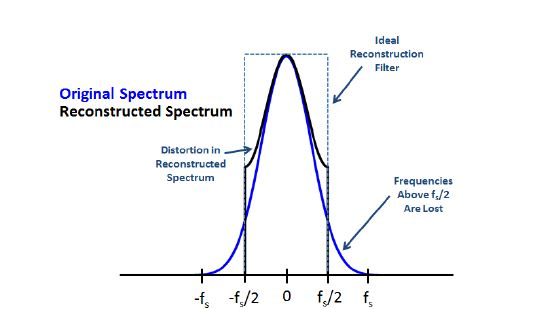
\includegraphics[width = 0.7\textwidth, frame]{Figures/Sampling/Folding_reconstruction}
\caption{Reconstructed Signal is Distorted}
\label{fig:Sampling:Folding_reconstruction}
\end{figure}

However, instead of getting back to the blue (original one), we end up with the black one. The black spectrum contains \tbi{2 type of distortion}:

\begin{enumerate}

\item Distortion due to folding (aliasing): the black amplitude values are the result from the summation of frequencies above and below $\pm\, \displaystyle\frac{F_s}{2}$, which fold back in the interval $\left[\, -\, \displaystyle\frac{F_s}{2} \, ; \, + \, \displaystyle\frac{F_s}{2} \, \right]$

\item Distortion due to the loss of high frequency content: the original blue spectrum does indeed have high frequency content above $\displaystyle\frac{F_s}{2}$ due to the uncertainty principle.

\end{enumerate}

\subsection{Anti-Aliasing Filter}

How can we fight the distortions introduced in \autoref{fig:Sampling:Folding_reconstruction}? \\

First let's talk about the aliasing distortion. We know that frequencies above $\displaystyle\frac{F_s}{2}$ will fold back to the original spectrum (as discussed in \autoref{fig:Sampling:Folding}), so what we can do is get off the frequencies above $\displaystyle\frac{F_s}{2}$ so they won't fold back when doing the reconstruction. In other words, we are limiting the signal to what it's called \tbi{effective bandwidth} when doing the cutting. Process is shown in \autoref{fig:Sampling:Anti_Aliasing_Filter}.

\begin{figure}[h]
\centering
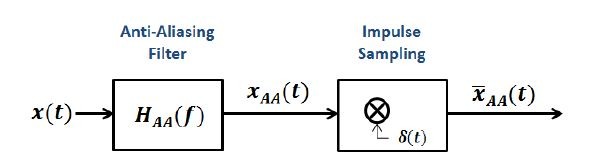
\includegraphics[width = 0.7\textwidth, frame]{Figures/Sampling/Anti_Aliasing_Filter}
\caption{Anti Aliasing Filter}
\label{fig:Sampling:Anti_Aliasing_Filter}
\end{figure}

\begin{itemize}

\item We have some time limited signal $x(t)$

\item We apply the anti-aliasing filter

\item Then we do impulse sampling

\end{itemize}

Result of this process is shown in \autoref{fig:Sampling:Anti_Aliasing_Filter_Result}.

\begin{figure}[h]
\centering
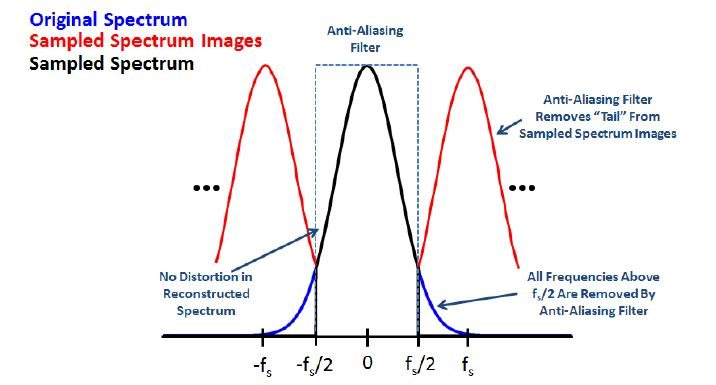
\includegraphics[width = 0.7\textwidth, frame]{Figures/Sampling/Anti_Aliasing_Filter_Result}
\caption{Anti Aliasing Filter: no folding frequencies}
\label{fig:Sampling:Anti_Aliasing_Filter_Result}
\end{figure}

\begin{itemize}

\item If we compare \autoref{fig:Sampling:Anti_Aliasing_Filter_Result} to \autoref{fig:Sampling:Folding}, we see that the tails shown in \autoref{fig:Sampling:Folding} of the replicated spectrum are gone now.

\item However, we did do a compromise, by throwing away the high frequency content above $\displaystyle\frac{F_s}{2}$.

	\begin{itemize}
	\item But this type of distortion can be controlled by increasing $F_s$ and hence throwing less of these high frequency content.
	
	\item So we need to do some engineering judgment about the choice of $F_s$ and the notion of effective bandwidth
\end{itemize}	  

\end{itemize}

\subsection{Practical Sampling with finite width pulse}

So far, we have done reconstruction using ideal train of pulse, which have no width at all. However,these type of pulses don't exist in reality, and the pulses which do exist are with finite width. So can we do the same math and reconstruction using these finite width pulses as we did with the ideal train of pulses ? 

The answer is yes we can and that's thanks to Fourier series as we will see later. 

First we develop the theory of these computations, then we take some practical example.\\

\underline{Theoretical Development:}\\

The steps of the theory are show in \autoref{fig:Sampling:practical_sampling} and \autoref{fig:Sampling:practical_sampling_2} 


\begin{figure}[h]
\centering
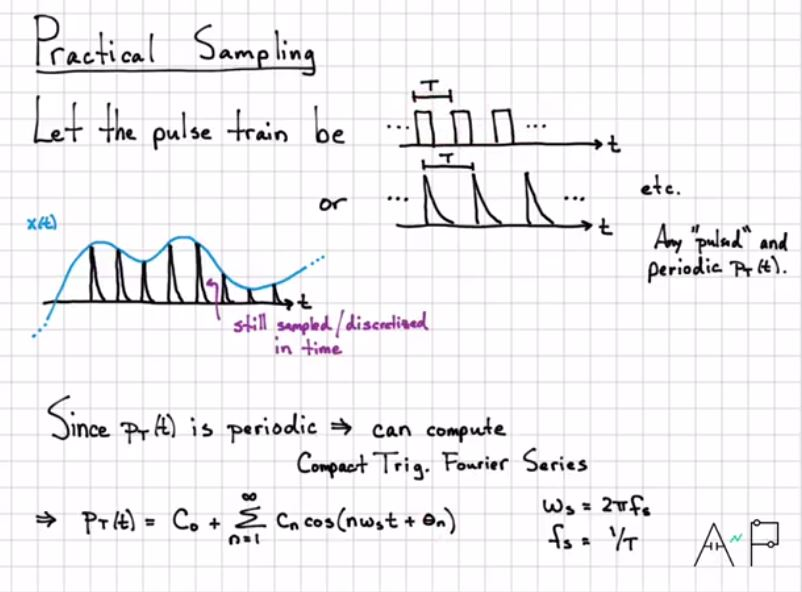
\includegraphics[width = 0.7\textwidth, frame]{Figures/Sampling/practical_sampling}
\caption{Practical Sampling using periodic finite width pulses}
\label{fig:Sampling:practical_sampling}
\end{figure}

\begin{itemize}

\item We can use any form of \tbi{periodic waveform} (square, triangular) of period $T_s$, denoted by $p_{T_s}(t)$ where $p$ stand for pulses

\item We multiply $x(t)$ by these periodic pulses, and hence we localize the signal at some discrete time interval as shown in 

\item Since the resultant of the multiplication is periodic signal, we can use the Fourier series (any form of Fourier Series, here we use the compact form)

\end{itemize}

\begin{figure}[h]
\centering
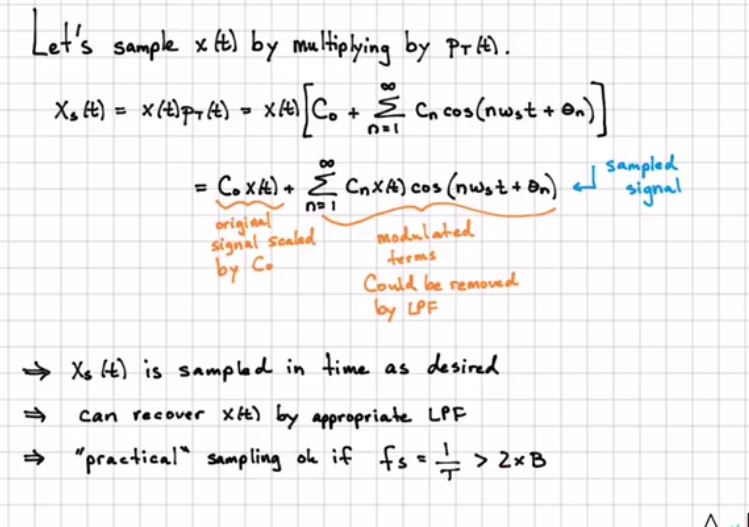
\includegraphics[width = 0.7\textwidth, frame]{Figures/Sampling/practical_sampling_2}
\caption{Practical Sampling using periodic finite width pulses: Fourier series}
\label{fig:Sampling:practical_sampling_2}
\end{figure}

\begin{itemize}

\item Notice that the signal is composed from 2 terms:

	\begin{enumerate}
	\item $C_0 \, x(t)$ which is the signal scaled by a factor $C_0$
	
	\item The modulated terms $\displaystyle\sum_{n \, = \, 1}^{+\,\infty} C_n \,\, x(t) \, \text{cos} \left( n \, \omega_s \, t \, + \, \theta_n  \right)$, which can be removed using low pass filter
	\end{enumerate}

\end{itemize}


\underline{Examples:}\\

Given are shown in \autoref{fig:Sampling:practical_sampling_example}.

\begin{figure}[h]
\centering
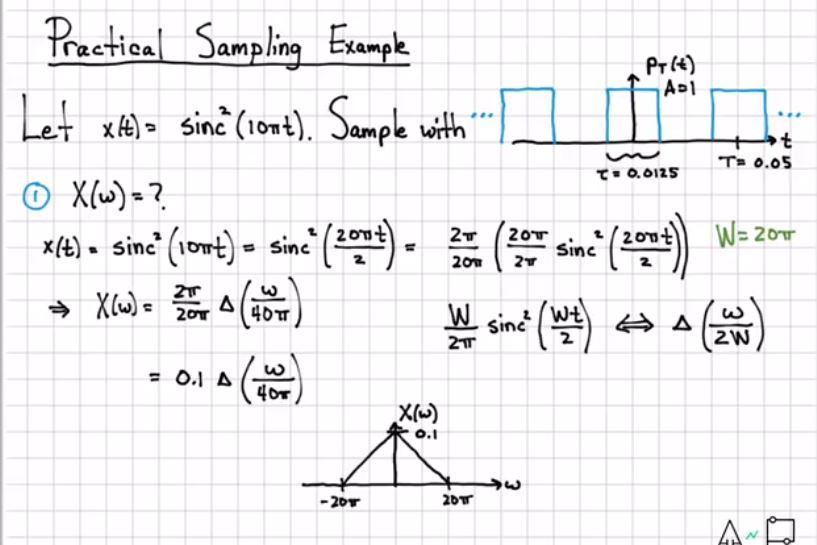
\includegraphics[width = 0.7\textwidth, frame]{Figures/Sampling/practical_sampling_example}
\caption{Practical Sampling Example}
\label{fig:Sampling:practical_sampling_example}
\end{figure}

\begin{itemize}

\item The periodic waveform we used for sampling is a square wave where the sampling period (period of the square wave) is $T_s \, = \, 0.05 $ s and pulse width $\tau \, = \, 0.0125 \, \text{s} \, = \, \displaystyle\frac{T_s}{4}$ 

\item $x(t) \, = \, \text{sinc}^2 (10 \pi t)$ has been reformulated so we can use a look up table to deduce $X(\omega)$ which is a triangular pulse of width $40 \pi$

\item Computation and development of Fourier series shown in \autoref{fig:Sampling:practical_sampling_example_compute}, \autoref{fig:Sampling:practical_sampling_example_compute_2} and \autoref{fig:Sampling:practical_sampling_example_compute_3}  


\begin{figure}[h]
\centering
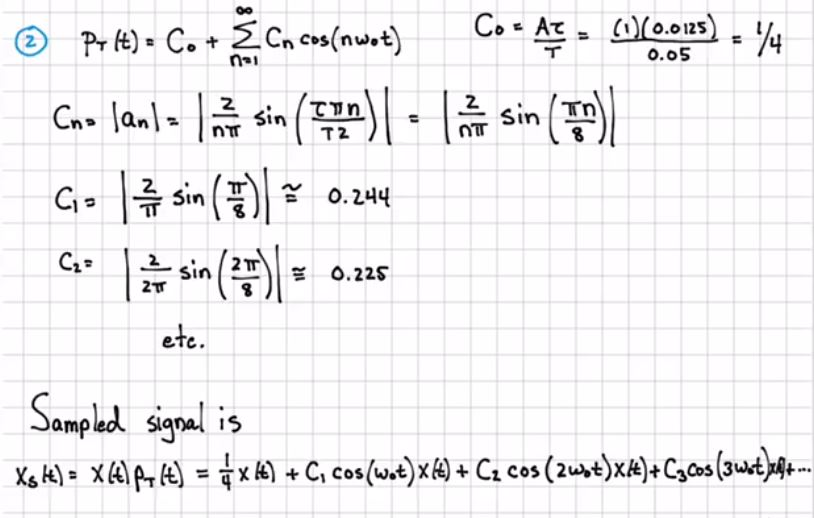
\includegraphics[width = 0.7\textwidth, frame]{Figures/Sampling/practical_sampling_example_compute}
\caption{Practical Sampling Example: Computing Fourier Series}
\label{fig:Sampling:practical_sampling_example_compute}
\end{figure}

	\begin{itemize}
	\item In \autoref{fig:Sampling:practical_sampling_example_compute}, first we develop the Fourier series of the square wave
	
	\item As a $\mathrm{2}^{nd}$ step, the sampled signal will be the product between $x(t)$ and train of square wave pulses $p_{T_s}(t)$.
	\end{itemize}

\newpage
\item Continue to expand $x_{\text{ZOH}}(t)$ (shown in \autoref{fig:Sampling:practical_sampling_example_compute_2}) where the cos is a dirac signal, and the multiplication in the time domain is a convolution in the frequency

\begin{figure}[h]
\centering
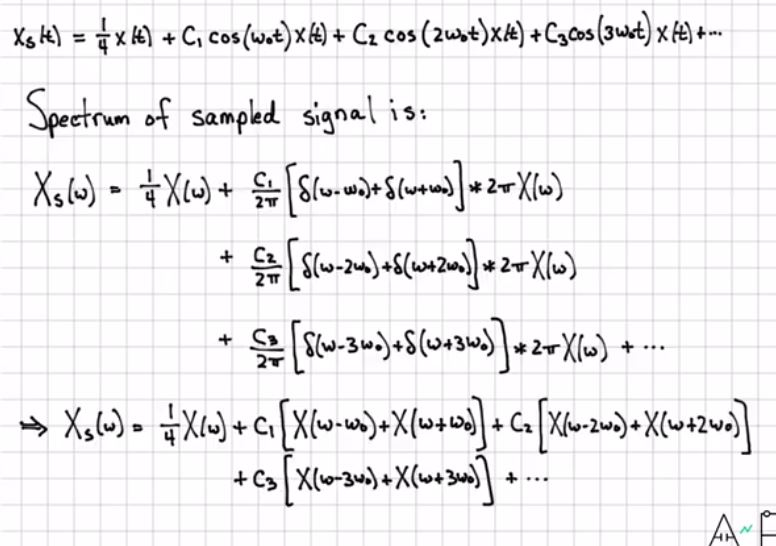
\includegraphics[width = 0.7\textwidth, frame]{Figures/Sampling/practical_sampling_example_compute_2}
\caption{Practical Sampling Example: Computing Fourier Series}
\label{fig:Sampling:practical_sampling_example_compute_2}
\end{figure}


	\begin{itemize}
	\item Then we use the convolution property of a signal with a dirac function
	\end{itemize}

\item Sketching the amplitude spectrum of $x_{\text{ZOH}}(t)$ (shown in \autoref{fig:Sampling:practical_sampling_example_compute_3})

\begin{figure}[h]
\centering
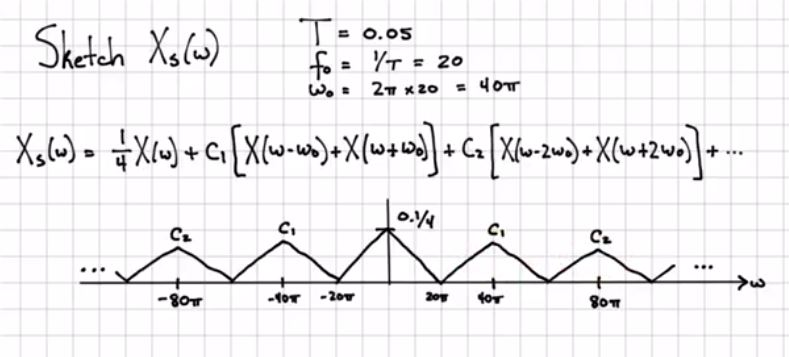
\includegraphics[width = 0.7\textwidth, frame]{Figures/Sampling/practical_sampling_example_compute_3}
\caption{Practical Sampling Example: Amplitude Spectrum of $x_{\text{ZOH}}(t)$}
\label{fig:Sampling:practical_sampling_example_compute_3}
\end{figure}

\end{itemize}




\newpage
\section{Ideal Reconstruction}

After we have seen the ideal sampling method, our goal now is to \tbi{undo the effect of sampling} and reconstruct back the continuous time signal.\\

Some people call this process \tbi{reconstruction} or \tbi{interpolation}.\\


It should be noted that the \tbi{results} developed \tbi{in this section} are \tbi{under the conditions that}:

\begin{enumerate}

\item The signal is in time is \tbi{not time limited} (so not truncation in time)

\item And its is \tbi{bandlimited}

\end{enumerate}

Practical sampling and reconstruction will be developed later in \autoref{Sec:Sampling:Practical_Sampling and_Reconstruction}.

\subsection{Sampling theorem and the Uniqueness of Reconstruction}

Suppose we have been given some set of discrete values as shown in  \autoref{fig:Sampling:example_reconstruction}.

\begin{figure}[h]
\centering
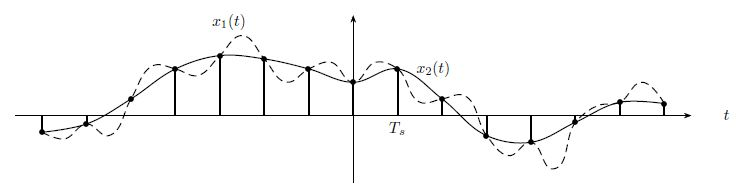
\includegraphics[width = 0.7\textwidth, frame]{Figures/Sampling/example_reconstruction}
\caption{Which signal is the correct one ?}
\label{fig:Sampling:example_reconstruction}
\end{figure}

There are many ways to plot a signal using these discrete values: one can plot and obtain $x_1(t)$ and another can obtain $x_2(t)$, so how can we ensure which signal is the correct one?\\

We can do this using the frequency representation of the sampling studied in the previous sections and using the sampling theorem, which is stated formally in \autoref{fig:Sampling:sampling_theorem_definition}.


\begin{figure}[h]
\centering
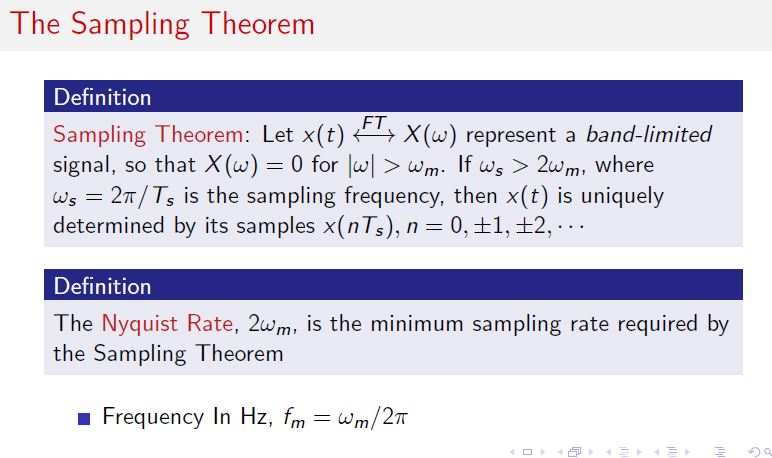
\includegraphics[width = 0.7\textwidth, frame]{Figures/Sampling/sampling_theorem_definition}
\caption{Sampling Theorem Definition}
\label{fig:Sampling:sampling_theorem_definition}
\end{figure}

\begin{itemize}

\item Notice that sampling theorem is for \tbi{band limited signal}

\item The sampling theorem give us an \tbi{upper bound} that we should sample at least from $2 \, \omega_m$ to avoid aliasing and reconstruct the signal back

\end{itemize}

\subsection{Ideal (Sinc) Interpolation}

Now we develop the mathematical model for reconstruction for impulse sampling case. Given that we have the impulse sampled spectrum as shown in \autoref{fig:Sampling:impulse_reconstruction}, how we can get back to the original spectrum ?

\begin{figure}[h]
\centering
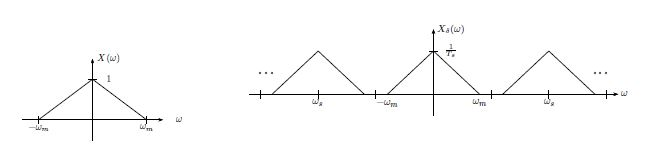
\includegraphics[width = 0.7\textwidth, frame]{Figures/Sampling/impulse_reconstruction}
\caption{Ideal Reconstruction: Spectrum of Original Signal and Impulse Sampled Signal}
\label{fig:Sampling:impulse_reconstruction}
\end{figure}

The answer is that we need to get rid off of the replicate at multiple of $\omega_s$, and then apply the proper gain for the filter because we have the scale factor $\displaystyle\frac{1}{T_s}$, and the original spectrum $X(\omega)$ has an max amplitude of 1 as shown in \autoref{fig:Sampling:impulse_reconstruction}.\\

The correspondent filter is shown in \autoref{fig:Sampling:Ideal_Reconstruction_Filter}.

\begin{figure}[h]
\centering
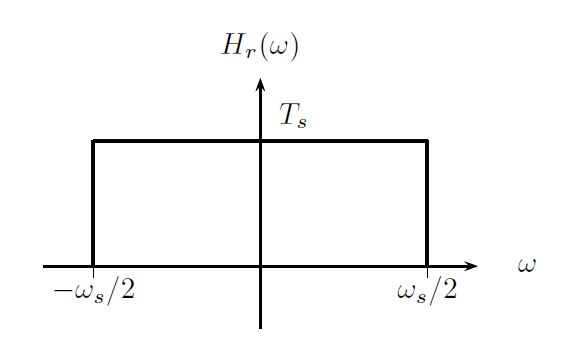
\includegraphics[width = 0.7\textwidth, frame]{Figures/Sampling/Ideal_Reconstruction_Filter}
\caption{Frequency Response of Ideal Reconstruction Filter}
\label{fig:Sampling:Ideal_Reconstruction_Filter}
\end{figure}

Now we have done the reconstruction in the frequency domain, the computations (shown in \autoref{fig:Sampling:Ideal_Reconstruction_Filter_time_domain_1} and \autoref{fig:Sampling:Ideal_Reconstruction_Filter_time_domain_2}) are also done in the time domain to understand what happens also, and how the reconstruction is done.

\begin{figure}[h]
\centering
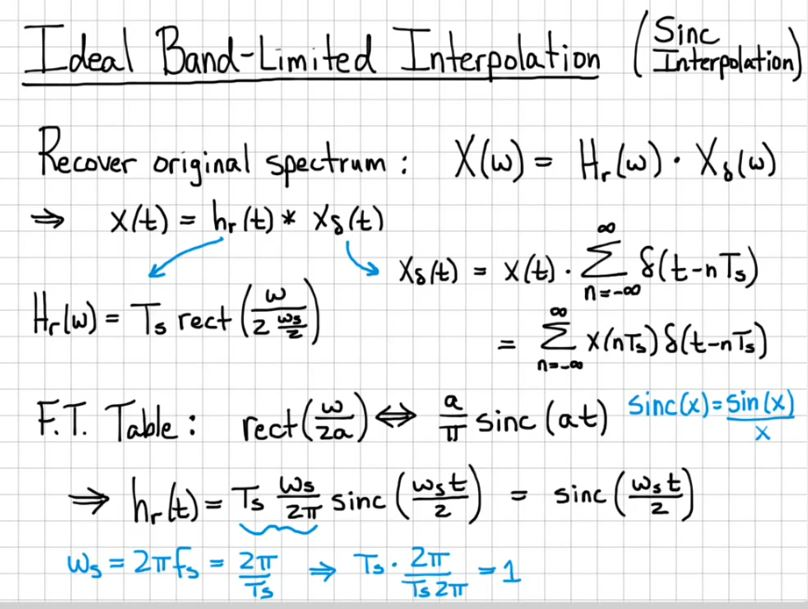
\includegraphics[width = 0.7\textwidth, frame]{Figures/Sampling/Ideal_Reconstruction_Filter_time_domain_1}
\caption{Computing $x(t)$ in the time domain starting from frequency domain formulation}
\label{fig:Sampling:Ideal_Reconstruction_Filter_time_domain_1}
\end{figure}


\begin{itemize}

\item We start from frequency domain formulation $X(\omega) \, = \, H_r(\omega) \, \times \, X_{\delta}(\omega)$


\item Multiplication in the frequency domain is convolution in the time domain

\item In $x_{\delta}(t)$, we can get $x(t)$ into the summation as $x(n \, T_s)$

\item We use some look up table to see what is $h_r(t)$.

\item Be aware to use the proper definition of $\text{sinc}(x)$

\end{itemize}


\newpage
Final form of $x(t)$ is shown in \autoref{fig:Sampling:Ideal_Reconstruction_Filter_time_domain_2}. 

\begin{figure}[h]
\centering
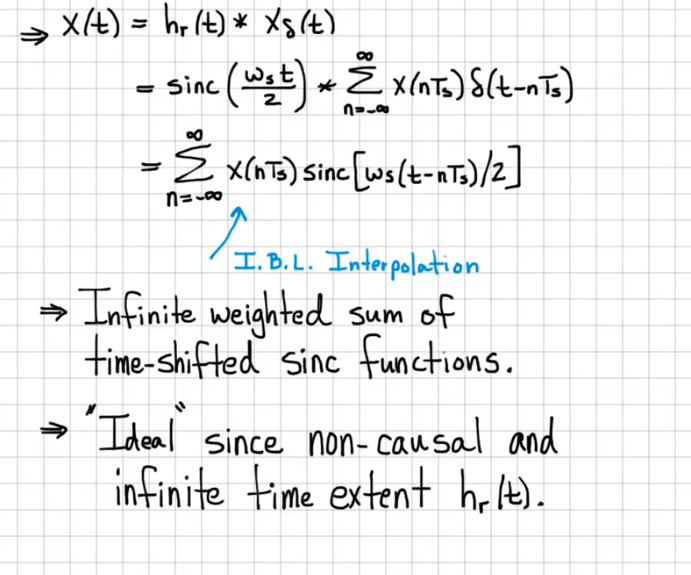
\includegraphics[width = 0.7\textwidth, frame]{Figures/Sampling/Ideal_Reconstruction_Filter_time_domain_2}
\caption{Expression of $x(t)$}
\label{fig:Sampling:Ideal_Reconstruction_Filter_time_domain_2}
\end{figure}


\begin{itemize}

\item When we multiply some signal by impulse, it will be the signal shifted to the location of the impulse

	\begin{itemize}
	\item So we get sinc into the summation and replace $t$ by $t \, - \, n\, T_s$
	
	\end{itemize}

\item So $x(t)$ is the sum of shifted sinc, each weighted by a different amplitude $x(n \, T_s)$.

\end{itemize}

\newpage
The term ideal is because the impulse response $h_r(t)$ is non causal (start before 0) and extent to infinity. A demonstration is shown in \autoref{fig:Sampling:Ideal_Reconstruction_Filter_time_domain_3}.

\begin{figure}[h]
\centering
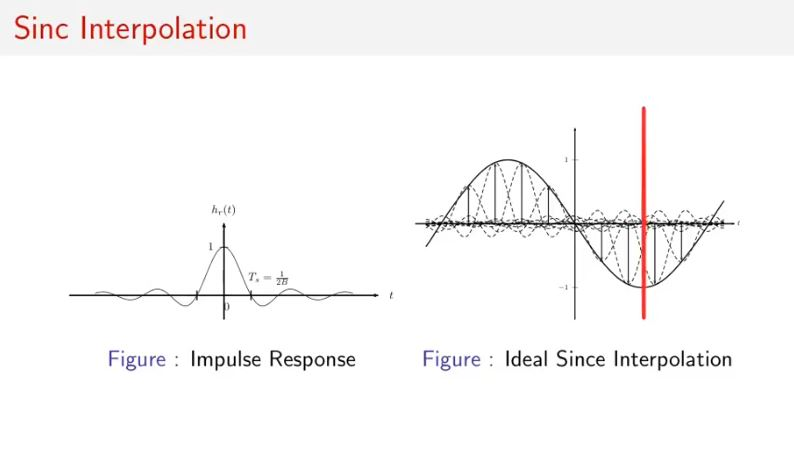
\includegraphics[width = 0.7\textwidth, frame]{Figures/Sampling/Ideal_Reconstruction_Filter_time_domain_3}
\caption{How the summation work}
\label{fig:Sampling:Ideal_Reconstruction_Filter_time_domain_3}
\end{figure}

\begin{itemize}

\item We have all these infinite sinc, and at a given time we sum all the values to obtain some value of $x(t)$.

\end{itemize}



\newpage
\section{Practical Sampling and Reconstruction}
\label{Sec:Sampling:Practical_Sampling and_Reconstruction}

Impulse sampling is one way we can get samples from the signal. Another way we can get samples is known as zero-order-hold (ZOH) as shown in \autoref{fig:Sampling:sampling_zoh}.

\begin{figure}[h]
\centering
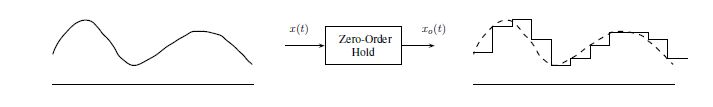
\includegraphics[width = 0.7\textwidth, frame]{Figures/Sampling/sampling_zoh}
\caption{Sampling using ZOH}
\label{fig:Sampling:sampling_zoh}
\end{figure}


It is named zero-order-hold because this filter grab a value of the signal, and then hold this value till it grab the next value. So the ZOH filter returns a stair case like signal, where each value of the signal is held till the next sampling time occurred.\\

Mathematical modeling of the ZOH is shown in \autoref{fig:Sampling:zoh_math}. 


\begin{figure}[h]
\centering
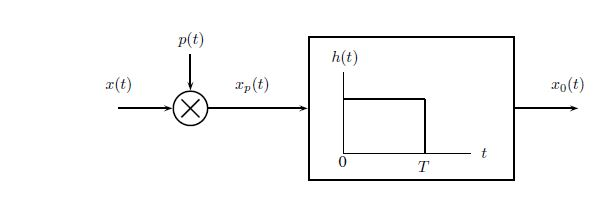
\includegraphics[width = 0.7\textwidth, frame]{Figures/Sampling/zoh_math}
\caption{Mathematical modeling of the ZOH}
\label{fig:Sampling:zoh_math}
\end{figure}


We have our continuous time signal $x(t)$ multiplied by an infinite train of pulse $p(t)$, then we obtain like before $x_p(t)$ which is equal to $x_{\delta}(t)$, then we do some low pass filtering using a pulse of width $T$. Amplitude spectrum of ZOH is shown in \autoref{fig:Sampling:zoh_amp_spectrum}. Recall that when we work in the digital domain, the only thing we care about is between $\pm \, \omega_s$.

\begin{figure}[h]
\centering
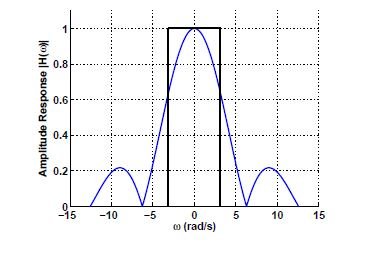
\includegraphics[width = 0.7\textwidth, frame]{Figures/Sampling/zoh_amp_spectrum}
\caption{Amplitude Spectrum of ZOH: boxed region is between $\pm \, \omega_s$}
\label{fig:Sampling:zoh_amp_spectrum}
\end{figure}


\underline{Spectrum of the Signal Compared to Impulse sampling of \autoref{fig:Sampling:impulse_sampling_spectrum_1}:}\\

Spectrum of the signal $x(t)$ using ZOH is shown in \autoref{fig:Sampling:zoh_output_spectrum}.

\begin{figure}[h]
\centering
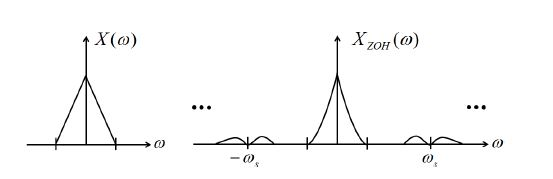
\includegraphics[width = 0.7\textwidth, frame]{Figures/Sampling/zoh_output_spectrum}
\caption{Output of ZOH in the frequency domain}
\label{fig:Sampling:zoh_output_spectrum}
\end{figure}

\begin{itemize}

\item In impulse sampling (see \autoref{fig:Sampling:impulse_sampling_spectrum_1}), the spectrum was the same (with the scale factor $\displaystyle\frac{1}{T_s}$), along with the replicate at multiple of $\omega_s$.


\item In ZOH, these replicate are attenuated due to the low pass nature of the ZOH, which is a good thing since we don't want these images.

\item However, the original spectrum is getting distorted, and this distortion is controlled by the time sampling we choose to get our values. 

\end{itemize}

\subsection{Mathematical Formulation for ZOH}

Ideal sampling followed by ideal bandlimited interpolation can't by done practically:

\begin{itemize}

\item Generating dirac pulses is very difficult

\item In reconstruction, the value of $\hat{y}(t)$ at a value of $t$ not multiple of $T_s$ is obtained by infinite sum of weighted sinc function

\item Ideal filters are also can't be made

\end{itemize}


ZOH is the practical way to grab a signal, which is done by taking a sample of the signal, and holding this value during the sampling interval.\\

Let's denote the rectangular pulse we are using by $h(t)$ denoted by:

\begin{equation}
h(t)\, = \, \begin{cases}
1 \quad 0 \, \leq \, t \, \leq \, T_s \\
0 \quad \text{otherwise}
\end{cases}
\end{equation}

The $x_{\text{zoh}}$ can be written as:

\begin{equation}
x_{\text{zoh}} \, = \, \displaystyle\sum\limits_{n \, = \, -\infty}^{\infty} x(n) h\left(	t \, - \, n\,T_s \right)
\label{Eq:Sampling:Zoh_eq_1}
\end{equation}

Recall that we can obtained a shifted version of a signal by convolving this signal with a dirac function so equation (\ref{Eq:Sampling:Zoh_eq_1}) can be further formulated:

\begin{equation}
\begin{array}{rcl}
x_{\text{zoh}} \, &=& \, \displaystyle\sum\limits_{n \, = \, -\infty}^{\infty} x(n) \, h\left(	t \, - \, n\,T_s \right) \\ \\		
&=& \, \displaystyle\sum\limits_{n \, = \, -\infty}^{\infty} x(n) \, \times \, \left[ \, \delta \left(	t \, - \, n\,T_s \right) \, * \, h(t) \, \right] \\ 
\end{array}
\label{Eq:Sampling:Zoh_eq_2}
\end{equation}


Manipulating the parenthesis of equation (\ref{Eq:Sampling:Zoh_eq_2}):

\begin{equation}
\begin{array}{rcl}
x_{\text{zoh}} \, &=& \, \displaystyle\sum\limits_{n \, = \, -\infty}^{\infty} x(n) \, h\left(	t \, - \, n\,T_s \right) \\ \\		
&=& \, \displaystyle\sum\limits_{n \, = \, -\infty}^{\infty} x(n) \, \times \, \left[ \, \delta \left(	t \, - \, n\,T_s \right) \, * \, h(t) \, \right] \\ \\
&=& \, \displaystyle\sum\limits_{n \, = \, -\infty}^{\infty} \left[\, x(n) \, \times  \, \delta \left(	t \, - \, n\,T_s \right) \, \right] \, * \, h(t)   \\ \\
&=& \,  x_{\delta}(t) \, * h(t)
\end{array}
\label{Eq:Sampling:Zoh_eq_3}
\end{equation}


Taking the Fourier transform of (\ref{Eq:Sampling:Zoh_eq_3}) we get:

\begin{equation}
\begin{array}{rcl}
X_{\text{zoh}}(\omega_c) \, &=& \, X_{\delta}(\omega_c) \, \times \, H(\omega_c) \\ \\
			 &=& \, \displaystyle\frac{1}{T_s} \, \displaystyle\sum\limits_{n  =  -\infty}^{\infty} X_a \left( \, \omega_c \, - \,  n \, \omega_s \right) \, \times \, 2 \, \text{exp}\left( \, -j \, \displaystyle\frac{\omega_c \, T_s}{2} \, \right) \, \times \, \text{sinc}\left(\, \displaystyle\frac{\omega_c \, T_s}{2} \,\right) 
\end{array}
\end{equation}

Since the rectangular pulse of \autoref{fig:Sampling:zoh_math} is not centered at 0, and it is shifted by $\displaystyle\frac{T_s}{2}$, we obtain a phase shift of $ 2 \, \text{exp}\left( \, -j \, \displaystyle\frac{\omega_c \, T_s}{2} \, \right)$ multiplying the sinc function.


\subsection{Reconstruction for ZOH}


Time delay by the factor of  $\displaystyle\frac{T_s}{2}$ can't be corrected, we have to deal with it. However, the distortion in original spectrum and the replication can be fixed.\\

\underline{Key notes in designing anti-imaging filter:}

\begin{itemize}

\item the key difficulty is in the transition band, where we need to suddenly pass to 0 in the stop band

\item This can be easily achieved if we have a high transition band, which implies that $\omega_s >> \,$ bandwidth signal

\item We later get back to this point when covering oversampling and undersampling, and how they can make the design of the anti-imaging filter less or more expensive.

\end{itemize}




\newpage
\section{Spectral Sampling}
\label{Sec:Sampling:Sepctral_Sampling}


After we have been dealing with the sampling theorem, which tells what are the minimum number of samples we need from the time domain to construct a correct waveform, we move now to the dual form, which is \tbi{sampling in the frequency domain} and derive the number of samples in the spectrum required to construct the time domain signal. We are expecting similar results due to the time-frequency duality we now from Fourier transform lessons.

Explanation shown in \autoref{fig:Sampling:sepctral_sampling_replication_time_signal}.


\begin{figure}[h]
\centering
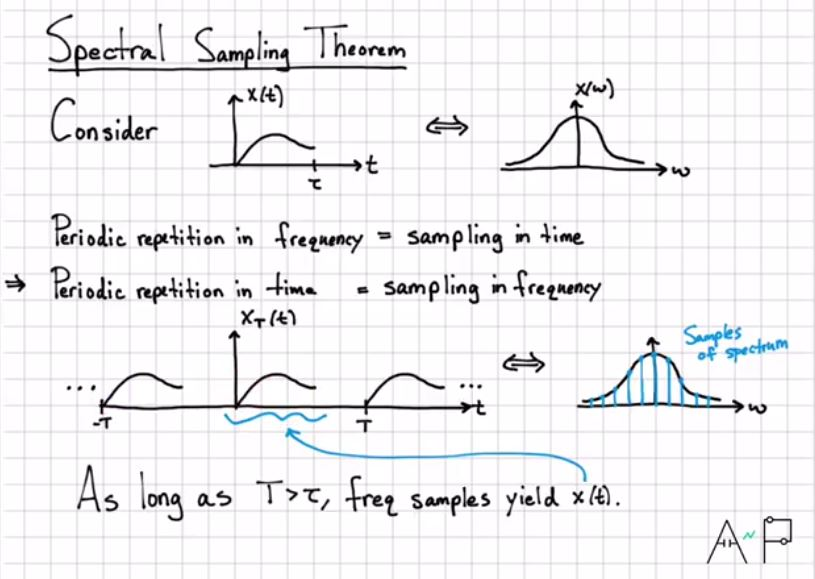
\includegraphics[width = 0.7\textwidth, frame]{Figures/Sampling/sepctral_sampling_replication_time_signal}
\caption{Replicating the time signal give us samples in the frequency domain}
\label{fig:Sampling:sepctral_sampling_replication_time_signal}
\end{figure}

\begin{itemize}

\item We are assuming we have a time limited domain signal $x(t)$ of duration $\tau$.

\item We know from \autoref{Sec:Sampling:Sampling_Continuous_Time_Signals} that sampling in time give us replication of the spectrum in the frequency domain

	\begin{itemize}
	\item The dual form now is that replicating in time give us samples in the frequency domain
	
	\item More generally, sampling in one domain give us replication in the $\mathrm{2}^{nd}$ domain
	\end{itemize}

\end{itemize}

\newpage
Now moving to deal with the mathematical development which relates the samples of $X(\omega)$ with $X(\omega)$ itself, shown in \autoref{fig:Sampling:sepctral_sampling_math_formulation}.


\begin{figure}[h]
\centering
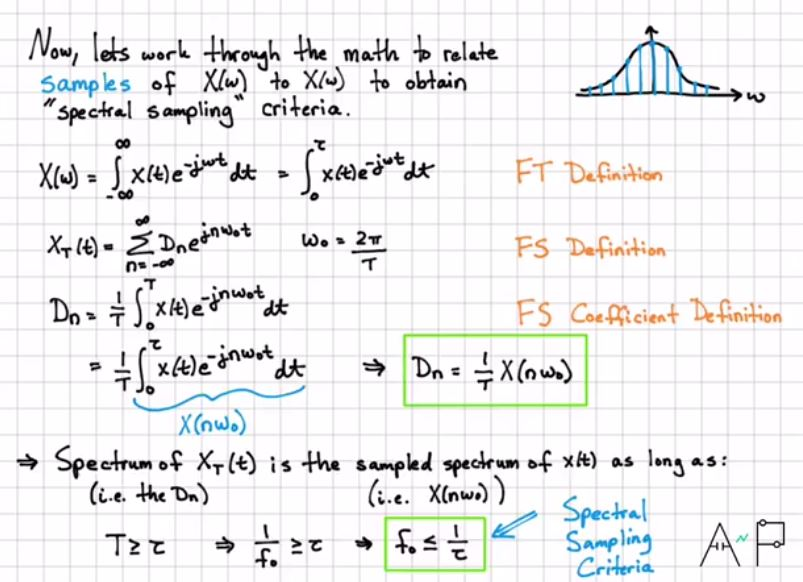
\includegraphics[width = 0.7\textwidth, frame]{Figures/Sampling/sepctral_sampling_math_formulation}
\caption{Mathematical formulation between samples of $X(\omega)$ and $X(\omega)$ itself}
\label{fig:Sampling:sepctral_sampling_math_formulation}
\end{figure}


\begin{itemize}

\item We start by Fourier transform definition

\item Since we are replicating in the time domain now, we can use Fourier series on $x_T(t)$

\item Notice the relation between $D_n$ and $X(\omega)$: they are the same except for the argument of the exponential:

	\begin{itemize}
	\item In $X(\omega)$, we have $\omega$
	
	\item In $D_n$, we have $n \, \omega_0$
	\end{itemize}

\end{itemize}

The \tbi{spectral sampling theorem} tells us: if we want to \tbi{describe a continuous time-limited signal} from its \tbi{spectrum samples}, we need to make sure that the \tbi{frequency spacing} $ \left(\, f_0 \, = \, \displaystyle\frac{1}{T} \, \right)$ is less than the inverse of the signal duration $\displaystyle\frac{1}{\tau}$







\section{Applications}


Sampling theorems let us replace a continuous time signal with a discrete set of numbers, so all we have to do now is to process these discrete numbers.\\ 

In this section we will look to some application of sampling, like how we can use the sample values to change the characteristic of a pulse.

A pulse can have different characteristics, like amplitude, width, position,$\cdots$. We start first by the following type of pulse modulation: PAM, PWM, PPM, and then treat PCM separately because it is the most sophisticated one among them.


\subsection{PAM, PWM and PPM}

\autoref{fig:Sampling:pulse_modulation} shows different type of pulse modulation

\begin{figure}[h]
\centering
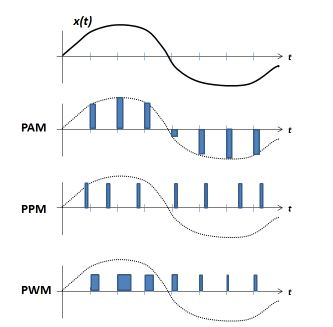
\includegraphics[width = 0.7\textwidth, frame]{Figures/Sampling/pulse_modulation}
\caption{Pulse Modulation}
\label{fig:Sampling:pulse_modulation}
\end{figure}

\begin{itemize}

\item In PAM: the more the sample value is higher, the amplitude of the pulse is higher

	\begin{itemize}
	\item The more the value is negative, same of the amplitude of the pulse
	\end{itemize}

\item In PPM, the width and amplitude of the pulses are all the same. However, the position of the pulse change

	\begin{itemize}
	\item If the value is more positive, the pulse become more early before the sample value
	
	\item If the value is negative, the pulse will be delayed and come after the sample value
	
	\item So we can now about sample value depending if the pulse arrive more early (more positive) or more delayed (more negative)
	\end{itemize}

\end{itemize}


\subsection{Quantization and A/D Process}

Before getting into PCM, we need to do learn some concepts whihc are prerequist to PCM. Let's start by some definitions:

\begin{itemize}

\item \tbi{Digital Signal:} discrete time signal and also discrete amplitude values

	\begin{itemize}
	\item Another definition of digital signal is that can be any continuous time signal which represents a stream of bits, like in PCM
\end{itemize}


\item \tbi{Quantization:} the process of rounding continuous valued amplitudes to a set of discrete amplitudes	

\begin{itemize}
\item Continuous-Time Signals Are Converted To Digital Signals By
Sampling and Quantizing (A/D converters do this)
\end{itemize} 

\item L-ary signal: A digital signal that can take on L different values

	\begin{itemize}
	\item Advantages of digital signal: resiliant to noise, use
of repeaters, error correction scheme more easy on digital signal (as opposite to continuous time signal which can take any value),
	\end{itemize}

\end{itemize}

\underline{Example of Quantization:}\\


\begin{figure}[h]
\centering
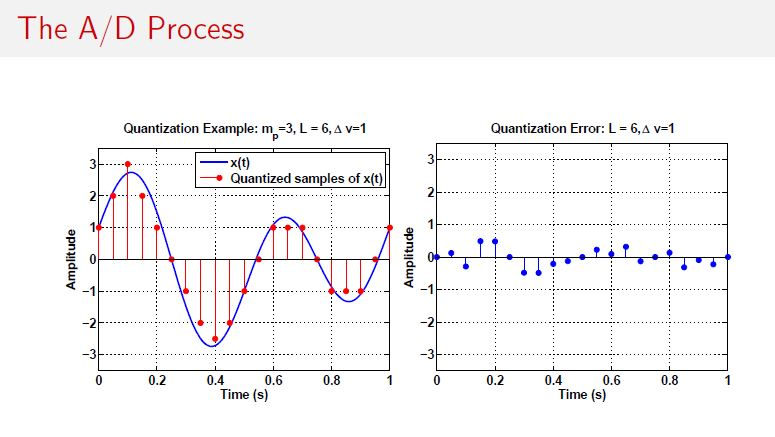
\includegraphics[width = 0.7\textwidth, frame]{Figures/Sampling/quantizaiton_example}
\caption{Quantization Example}
\label{fig:Sampling:quantizaiton_example}
\end{figure}


\begin{itemize}

\item In A/D process, first we sample the signal then we round up the value to a defined level

\item The parameters of the quantization (rounding) are:

	\begin{enumerate}
	\item The number of levels $L$: here we have 6 levels
	
	\item The step size between each level $\delta v$
	
	\item The peak value of the signal $m_p$
	\end{enumerate}


\newpage
\item Now \tbi{rounding introduce errors}, known here as \tbi{quantization error}

	\begin{itemize}
	\item If we want to decrease the quantization error, we need to increase the number of levels $L$ as \autoref{fig:Sampling:quantizaiton_example_2}
	
	\item However we need to allocate more bits to represents all of these levels (trade off)
	
	
	\begin{figure}[h]
\centering
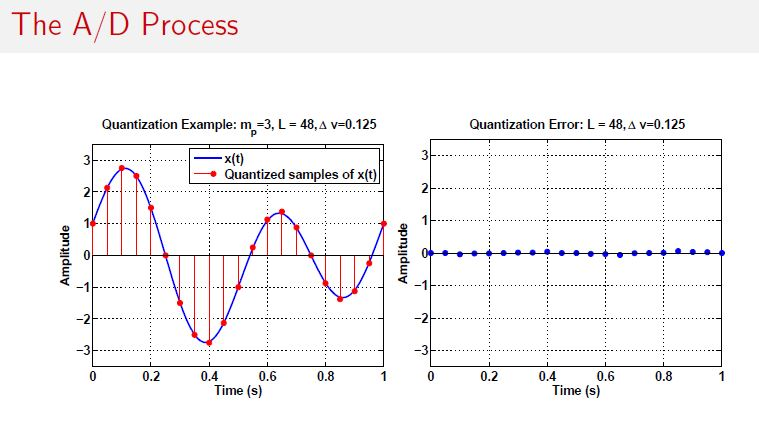
\includegraphics[width = 0.7\textwidth, frame]{Figures/Sampling/quantizaiton_example_2}
\caption{Increasing number of levels $L$ to decrease quantization error}
\label{fig:Sampling:quantizaiton_example_2}
\end{figure}
	
	\end{itemize}

\end{itemize}


\subsection{PCM}

PCM is a modulation scheme where we represent a stream of bits (after sampling and quantizing) into a sequence of pulses. An example is shown in \autoref{fig:Sampling:pcm_modulation}


\begin{figure}[h]
\centering
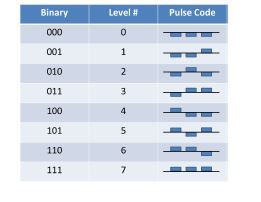
\includegraphics[width = 0.7\textwidth, frame]{Figures/Sampling/pcm_modulation}
\caption{PCM modulation using $L \, = \, 8$ levels}
\label{fig:Sampling:pcm_modulation}
\end{figure}

\begin{itemize}

\item After finishing the A/D process, we do mapping to these discrete numbers into a stream of bits


\item The the stream of bits is represented using pulses

	\begin{itemize}
	\item 1 using an positive pulse and 0 using a negative pulse
	\end{itemize}

\end{itemize}

\section{Practical Digital Filtering and Oversampling}


\begin{figure}[h]
\centering
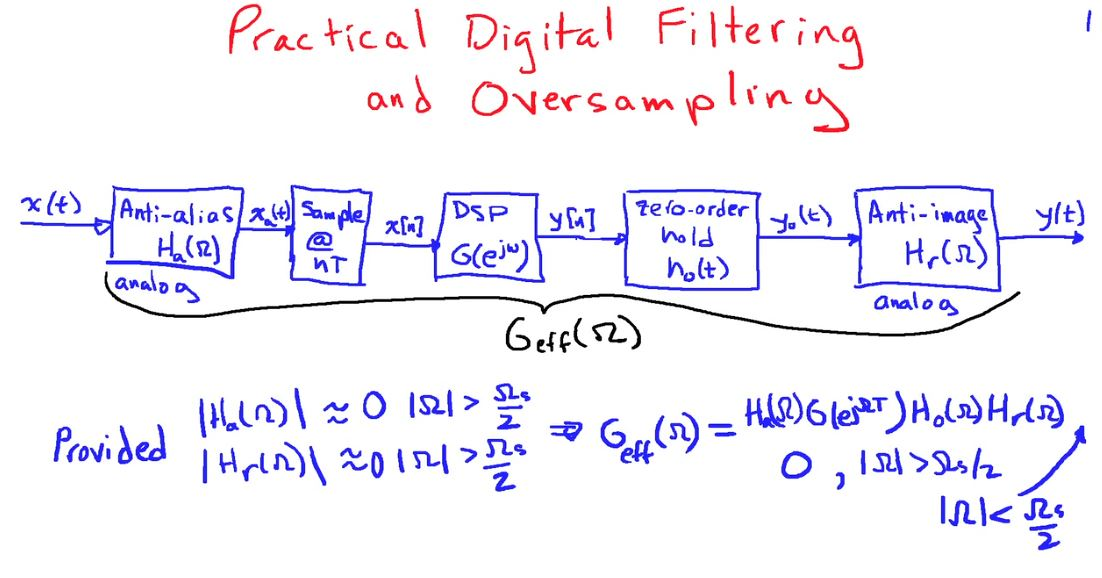
\includegraphics[width = 0.7\textwidth, frame]{Figures/Sampling/overall_sampling_reconstruction}
\caption{Overall Sampling and Reconstruction process}
\label{fig:Sampling:overall_sampling_reconstruction}
\end{figure}

\begin{itemize}

\item The DSP system is in the discrete frequency domain $\omega_d$

\end{itemize}

We can replace the whole system by a equivalent analog filter called $G_{\text{eq}}(\omega_c)$ where the transfer function is the multiplication of each transfer function block.

\subsection{Building Analog filters}


There are 2 filters presented in \autoref{fig:Sampling:overall_sampling_reconstruction} which are both \tbi{analog}: the anti-aliasing filter $H_{\text{ant}}(\omega_c)$ which cut high frequency to \tbi{prevent folding} and anti-imaging filter $H_{\text{ant-img}}(\omega_c)$ to \tbi{smooth the signal} after the ZOH operation.\\




\begin{itemize}

\item  For the anitliasing filter: if $\displaystyle\frac{\omega_s}{2}$ is close to the bandwidth of the signal $\omega_{\text{signal}}$, this means that the \tbi{transition band} of the filter is \tbi{very narrow} and that's \tbi{hard to implement in analog filters}.


\item For the anti-imaging filter: in the pass-band of the filter, we need to implement the inverse of the sinc to compensate the distortion made by the main lobe of the ZOH filter.

We need to make $\omega_s$ larger compared to the bandwidth of the signal so we don't have narrow band transition and the pass band 

\end{itemize}


So in summary, we need a high sampling rate. But in implementation, this comes at the cost excessive memory storage, because if my sampling rate is high, I have more data to process in a 1s, which means we need more memory for the storage.\\

So there is a trade-off between a high sampling rate and the memory needed for storage.

As a solution, we will change the sampling rate in the system of \autoref{fig:Sampling:overall_sampling_reconstruction}:

\begin{itemize}

\item Decrease the sampling rate after the ADC process, right before the discrete processing

\item Increase the sampling rate right before the ZOH

\end{itemize}


The new process including upsampling and downsampling is shown in \autoref{fig:Sampling:up_down_sampling}. 


\begin{figure}[h]
\centering
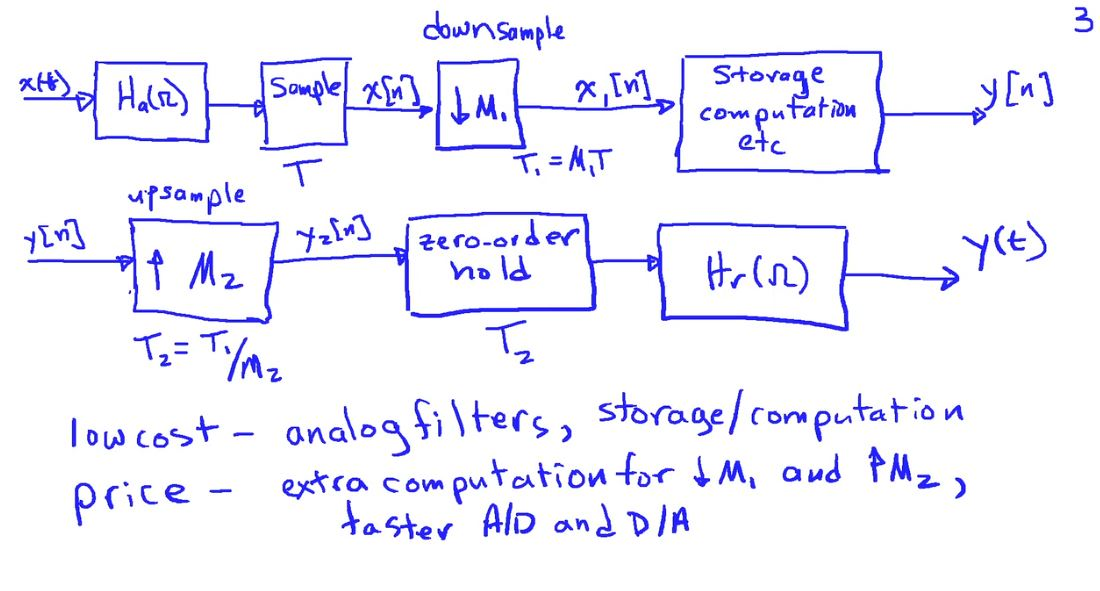
\includegraphics[width = 0.7\textwidth, frame]{Figures/Sampling/up_down_sampling}
\caption{Upsampling and downsampling for lower cost analog filters}
\label{fig:Sampling:up_down_sampling}
\end{figure}


\begin{itemize}

\item There are many efficient numerical methods to implement the up and down sampling operations

\item The price we pay in these discrete operations is worthy and make the design of the analog filters (anti-aliasing and anti-imaging) less expensive

\end{itemize}

\newpage
\subsection{Example of Oversampling}


Given are shown in \autoref{fig:Sampling:example_oversampling}.

\begin{figure}[h]
\centering
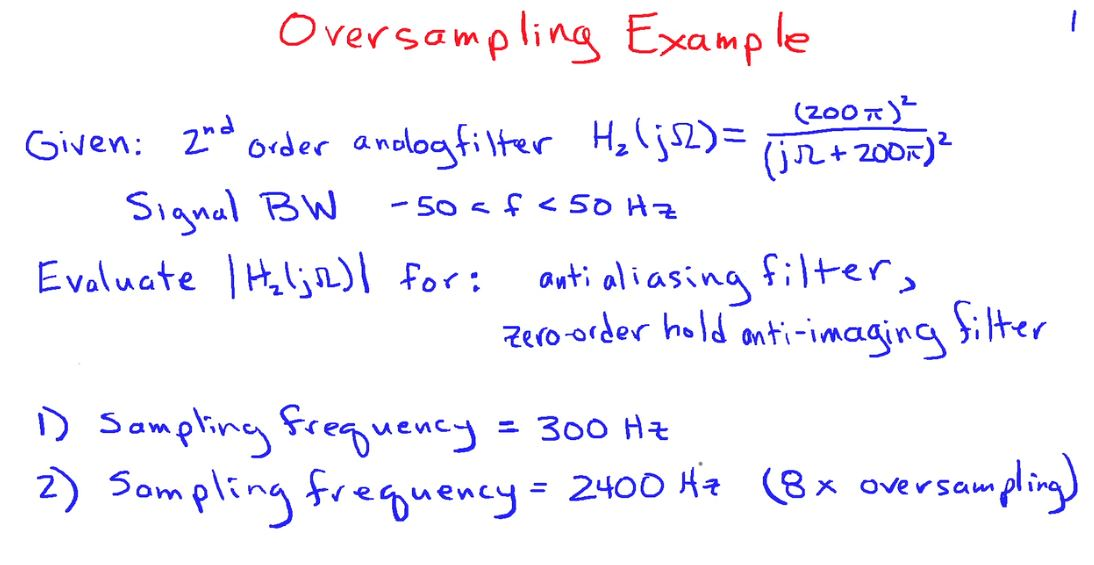
\includegraphics[width = 0.7\textwidth, frame]{Figures/Sampling/example_oversampling}
\caption{Given Example for oversampling}
\label{fig:Sampling:example_oversampling}
\end{figure}


The goal of this exercise is to show how oversampling can serve the analog filters (anti-aliasing and anti-imaging).


\begin{itemize}

\item The filter is an analog $\mathrm{2}^\mathrm{nd}$ order filter

\item The signal bandwidth is 50 Hz.

\item 2 sampling rate which both satisfy the Nyquist rate will be tested

\end{itemize}

\underline{Solution:}\\

\begin{enumerate}

\item For the anti-aliasing filter: \\

\begin{figure}[h]
\centering
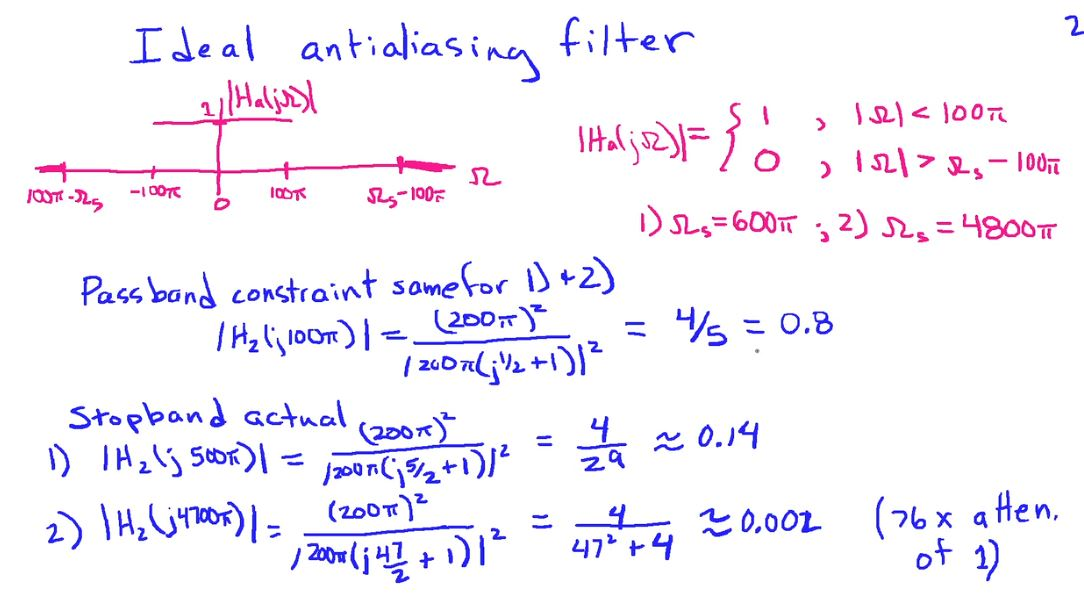
\includegraphics[width = 0.7\textwidth, frame]{Figures/Sampling/example_oversampling_sol_1}
\caption{Anti-aliasing filter solution}
\label{fig:Sampling:example_oversampling_sol_1}
\end{figure}

	\begin{itemize}
	
	\item The ideal anti-aliasing filter has an amplitude response of 1 in the pass-band and 0 in the stop band.
	
	\item Then we plug the computation for both $\omega_s$ and see the results	
	
	\begin{itemize}
	\item in the pass-band, the filtering is independent from $\omega_s$ so for both sampling rate, we have $ \mid H_{\text{ant-alias}}(\omega_c) \mid \, = \, 0.8$
	
	\item In the stop band we have the difference because the stop-band depend on $\omega_s$
	
	\end{itemize}
	
	\end{itemize}


 \item For the anti-imaging filter:

\begin{figure}[h]
\centering
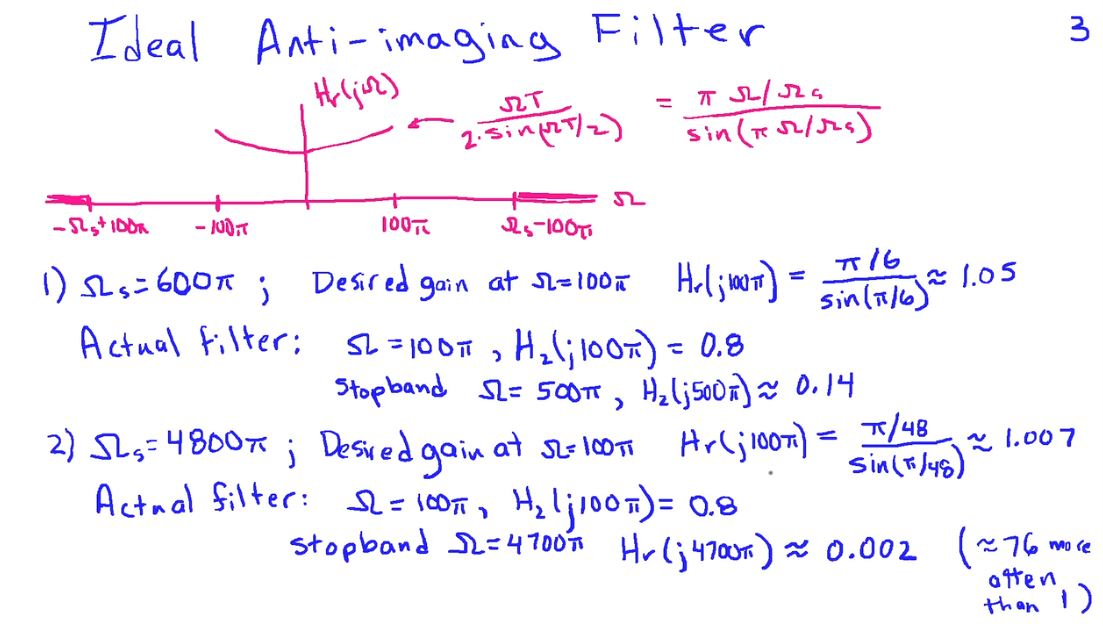
\includegraphics[width = 0.7\textwidth, frame]{Figures/Sampling/example_oversampling_sol_anti_imaging}
\caption{Anti-imaging filter solution}
\label{fig:Sampling:example_oversampling_sol_anti_imaging}
\end{figure}

\begin{itemize}

\item The ideal anti-imaging filter has the inverse of the sinc function as a frequency response


\item Also, the benefit is in the stop band, where oversampling is giving us more attenuation then the $ F_s \, = \,300 $ Hz

\end{itemize}

\end{enumerate}

\newpage
\subsection{Oversampling in D/A}

\autoref{fig:Sampling:oversampling_benefits} shows the D/A process.

\begin{figure}[h]
\centering
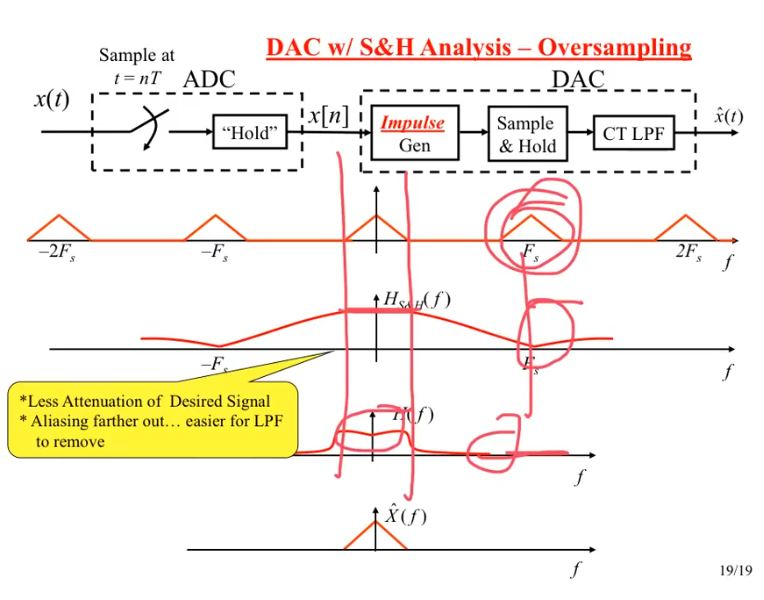
\includegraphics[width = 0.7\textwidth, frame]{Figures/Sampling/oversampling_benefits}
\caption{Over sampling Benefits}
\label{fig:Sampling:oversampling_benefits}
\end{figure}

Oversampling have several benefits:

\begin{itemize}

\item Make the frequency response of the ZOH system more flat in the pass band

\item Easier transition band design for the smoothing filter

\end{itemize}


\newpage

\section{Quantization and A/D Process}

In this section, we study quantization and its error.

\underline{Reminder:}\\

\begin{itemize}

\item \tbi{Digital Signal:} discrete time signal and also discrete amplitude values

	\begin{itemize}
	\item Another definition of digital signal is that can be any continuous time signal which represents a stream of bits, like in PCM
\end{itemize}


\item \tbi{Quantization:} the process of rounding continuous valued amplitudes to a set of discrete amplitudes	

\begin{itemize}
\item Continuous-Time Signals Are Converted To Digital Signals By
Sampling and Quantizing (A/D converters do this)
\end{itemize} 

\item L-ary signal: A digital signal that can take on L different values

	\begin{itemize}
	\item Advantages of digital signal: resiliant to noise, use
of repeaters, error correction scheme more easy on digital signal (as opposite to continuous time signal which can take any value),
	\end{itemize}

\end{itemize}

\underline{Example of Quantization:}\\


\begin{figure}[h]
\centering
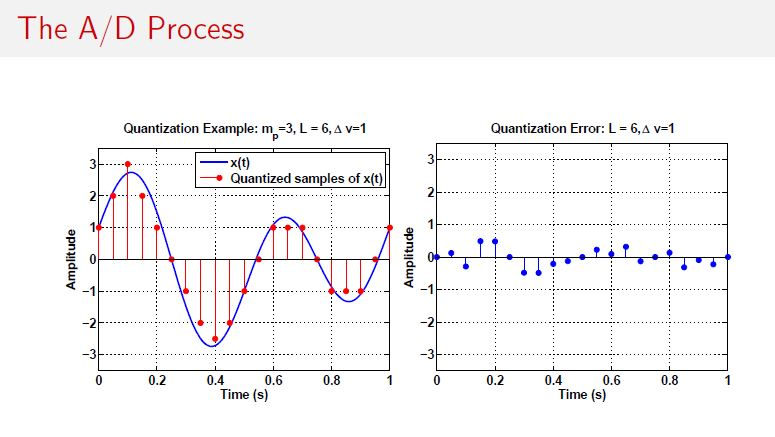
\includegraphics[width = 0.7\textwidth, frame]{Figures/Sampling/quantizaiton_example}
\caption{Quantization Example}
\label{fig:Sampling:quantizaiton_example}
\end{figure}


\begin{itemize}

\item In A/D process, first we sample the signal then we round up the value to a defined level

\item The parameters of the quantization (rounding) are:

	\begin{enumerate}
	\item The number of levels $L$: here we have 6 levels
	
	\item The step size between each level $\delta v$
	
	\item The peak value of the signal $m_p$
	\end{enumerate}


\newpage
\item Now \tbi{rounding introduce errors}, known here as \tbi{quantization error}

	\begin{itemize}
	\item If we want to decrease the quantization error, we need to increase the number of levels $L$ as \autoref{fig:Sampling:quantizaiton_example_2}
	
	\item However we need to allocate more bits to represents all of these levels (trade off)
	
	
	\begin{figure}[h]
\centering
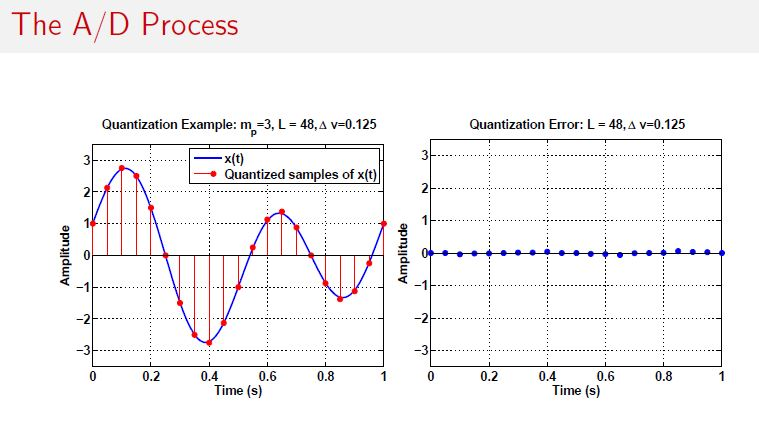
\includegraphics[width = 0.7\textwidth, frame]{Figures/Sampling/quantizaiton_example_2}
\caption{Increasing number of levels $L$ to decrease quantization error}
\label{fig:Sampling:quantizaiton_example_2}
\end{figure}
	
	\end{itemize}

\end{itemize}


\underline{Qunatization Formula:}

\begin{equation}
x_{\text{qunatized}} \, = \, \text{round} \left(\, \displaystyle\frac{x}{\text{step size}}\, \right) \, \times \, \text{step size}
\end{equation}


\newpage
\subsection{Dynamic Range of an Ideal ADC}

\begin{figure}[h]
\centering
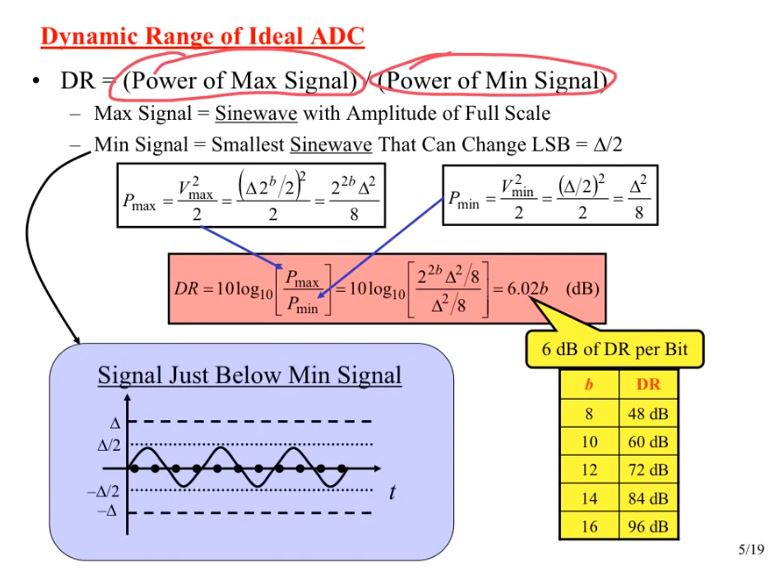
\includegraphics[width = 0.7\textwidth, frame]{Figures/Sampling/dynamic_range_ideal_adc}
\caption{Dynamic Range of an Ideal ADC}
\label{fig:Sampling:dynamic_range_ideal_adc}
\end{figure}


\subsection{Error Analysis of the Quantization Error}

Since qunantization error is unpredictable, we use statistical analysis and probability laws to describe the error.


\begin{equation}
\begin{array}{rcl}
e_q[k] \, &=& \, x[k] \, - \, x_q[k] \\\\
\displaystyle\frac{- \text{step}}{2} &\leq \, e_q[k] \, &\leq \, \displaystyle\frac{+ \text{step}}{2} \\ \\
\text{step} \, &=& \, \displaystyle\frac{\text{Range}}{\text{nb of Levels}} \\ \\
&=& \, \displaystyle\frac{\text{Range}}{2^{\left(\,\text{nb of bits + 1} \, \right)}  }
\end{array}
\end{equation}


\newpage
Error Analysis is shown in \autoref{fig:Sampling:quantizaiton_error_analysis}.

\begin{figure}[h]
\centering
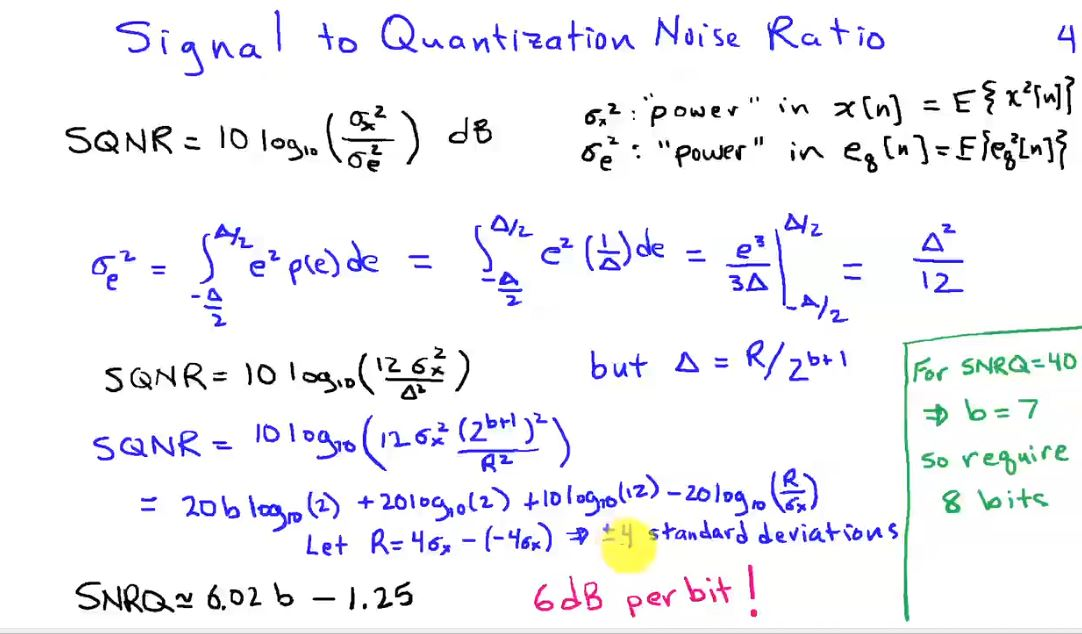
\includegraphics[width = 0.7\textwidth, frame]{Figures/Sampling/quantizaiton_error_analysis}
\caption{Qunatization Error Analysis}
\label{fig:Sampling:quantizaiton_error_analysis}
\end{figure}

\begin{itemize}

\item 

\begin{equation}
\begin{array}{rcl}
\text{SNQR} 	\, &=& \, 10 \, \text{log}_{10} \left(\, \displaystyle\frac{\sigma_x^2}{\sigma_e^2} \, \right) \\ \\
			& \approx & \, 6.02 \, - \, 1.25 \text{ dB/bit}		
\end{array}
\end{equation}


\item The analysis done is under particular assumptions for this statistical analysis:

	\begin{enumerate}
	\item $e_q[k]$ is a stationary random process with a uniform continuous distribution 
	
	\item $e_q[k]$ values are uncorrelated
	
	\item $e_q[k]$ and $x[k]$ are independent 
	\end{enumerate}

\end{itemize}


\newpage
In \autoref{fig:Sampling:quantizaiton_error_example}, we have an example of quantized and non-quantized sin.



\begin{figure}[h]
\centering
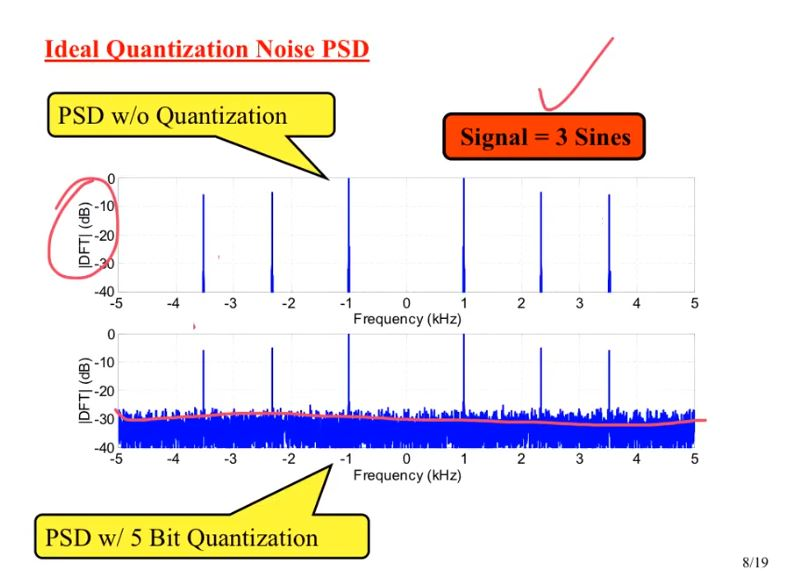
\includegraphics[width = 0.7\textwidth, frame]{Figures/Sampling/quantizaiton_error_example}
\caption{Qunatization Error Example}
\label{fig:Sampling:quantizaiton_error_example}
\end{figure}


\begin{itemize}

\item We can see that the power sepctral density in the quantized part is flat over all the frequency ranges


\item If we use fewer bit in the quantization process, the noise floor will get up

\end{itemize}


\newpage
\underline{SNQR for Full Scale Sine wave:}\\

\begin{figure}[h]
\centering
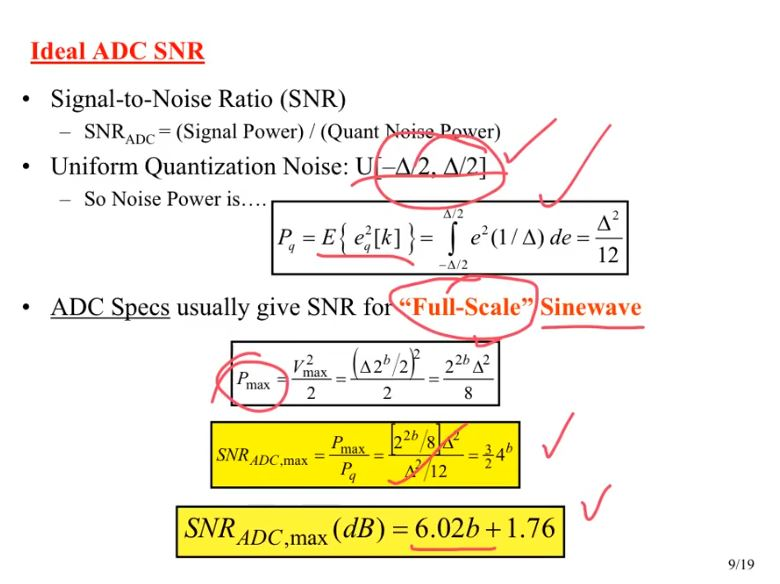
\includegraphics[width = 0.7\textwidth, frame]{Figures/Sampling/snr_full_sin_wave}
\caption{SNR for full sin wave}
\label{fig:Sampling:snr_full_sin_wave}
\end{figure}


\begin{itemize}
\item The SNQR in \autoref{fig:Sampling:snr_full_sin_wave} is a little bit optimistic because we are assuming a full range for the sin wave
\end{itemize}

We can generalize more the SNQR as in \autoref{fig:Sampling:snr_peak_factor}, where use the idea of peak factor to see the exact SNQR.


\newpage
\begin{figure}[h]
\centering
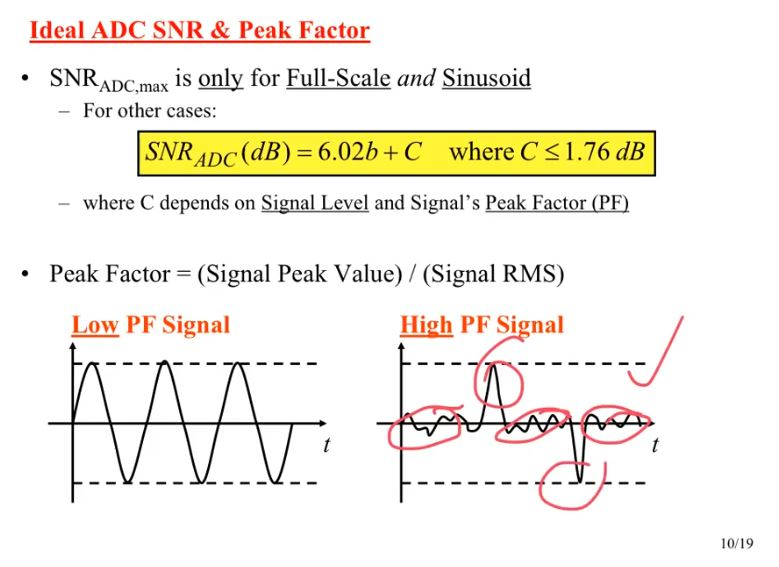
\includegraphics[width = 0.7\textwidth, frame]{Figures/Sampling/snr_peak_factor}
\caption{SNR and peak factor}
\label{fig:Sampling:snr_peak_factor}
\end{figure}

\autoref{fig:Sampling:snr_peak_factor_relation} shows the relation of SNQR and peak factor in dB.


\begin{figure}[h]
\centering
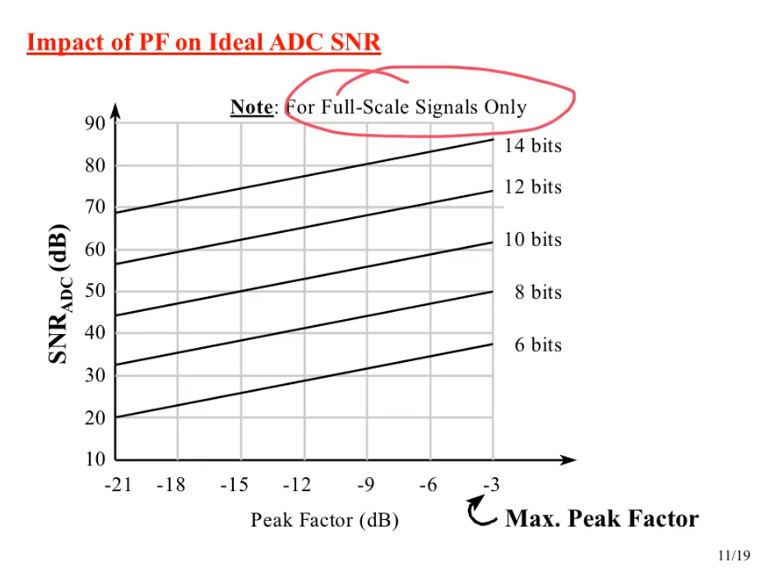
\includegraphics[width = 0.7\textwidth, frame]{Figures/Sampling/snr_peak_factor_relation}
\caption{SNR and peak factor relation}
\label{fig:Sampling:snr_peak_factor_relation}
\end{figure}

\begin{itemize}
\item The more the signal is peaky for a fixed number of bits, the more SNQR is low
\end{itemize}


\subsection{More Source of Errors}

\autoref{fig:Sampling:more_error} shows more sources of errors we can get

\begin{figure}[h]
\centering
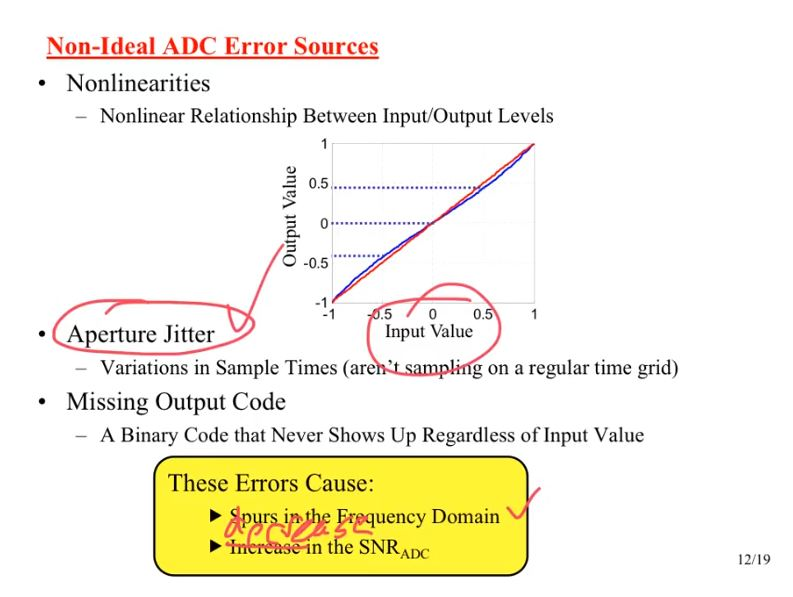
\includegraphics[width = 0.7\textwidth, frame]{Figures/Sampling/more_error}
\caption{SNR and peak factor relation}
\label{fig:Sampling:more_error}
\end{figure}

\begin{itemize}

\item Jitter: comes from clock circuitry we use to do the sampling


\item These errors also shows decrease in the SNQR

\end{itemize}

\autoref{fig:Sampling:spurse} shows how the spruse comes into the amplitude spectrum plots in addition to the noise floor.

\begin{figure}[h]
\centering
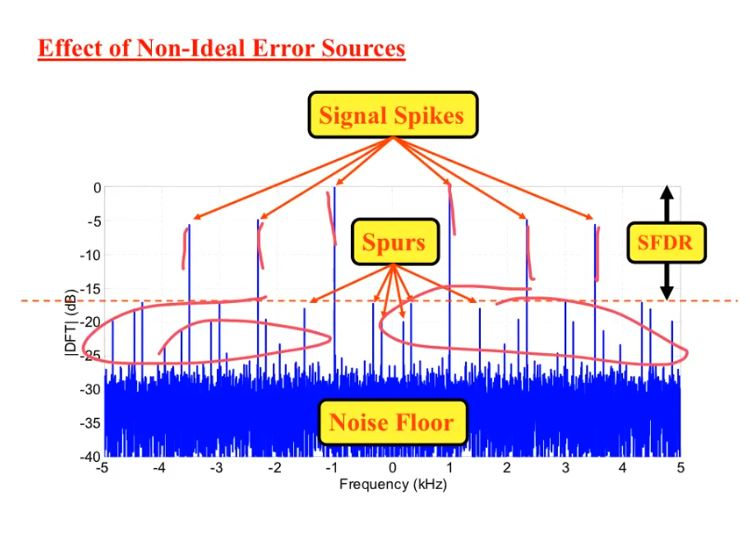
\includegraphics[width = 0.7\textwidth, frame]{Figures/Sampling/spurse}
\caption{Spurse Errors in the Spectrum}
\label{fig:Sampling:spurse}
\end{figure}

\begin{itemize}
\item SFDR set the distance between the actual signals and the spurse
\end{itemize}


\subsection{Specs for ADC}

\begin{figure}[h]
\centering
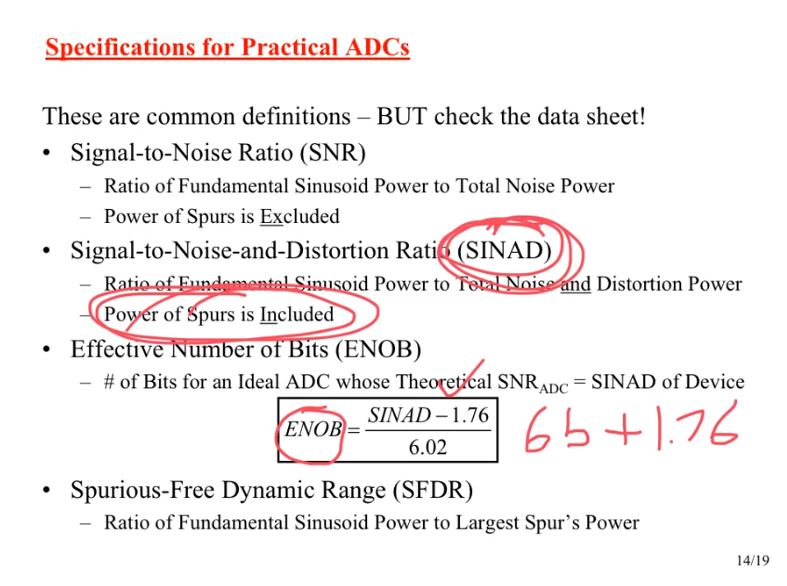
\includegraphics[width = 0.7\textwidth, frame]{Figures/Sampling/ADC_Specs}
\caption{Most common specfication on ADC}
\label{fig:Sampling:ADC_Specs}
\end{figure}

\begin{itemize}

\item ENOB: take into consideration the actual number of bits due SINAD (spurse errors)

	\begin{itemize}
	\item It is the algebraic solution of $\text{SINAD} \, = \, 6 \, \text{bits} \, + \, 1.76$
	
	\item Due to hardware imperfections (spurse), in theory we could have 8 bits, but in reality it may comes down in to 6 bits
	\end{itemize}

\end{itemize}



\newpage
\section{Oversampling and $\Sigma-\Delta$ Converter}

We have seen that oversampling have several advantages. Now let's relate the oversampling to the SNQR.



\begin{itemize}

\item Since we are sampling much higher than the signal bandwidth, we can assume that the signal bandwidth is small compared to $\displaystyle\frac{F_s}{2}$, and the spectrum reside in a small region of the interval $\left[\, \displaystyle\frac{- F_s}{2} \, ; \, \displaystyle\frac{+ F_s}{2} \right] $


\item So we have less noise in the signal spectrum $\rightarrow$ SNQR improve


\item So also ENOB improves

	\begin{itemize}
	\item However at the cost of a higher $F_s$
	\end{itemize}

\item But this is an inefficient trade-off: because we obtain 1 bit per 6 dB

	\begin{itemize}
	\item Computation shown in \autoref{fig:Sampling:oversampling_SNQR_relation}
	
	\begin{figure}[h]
\centering
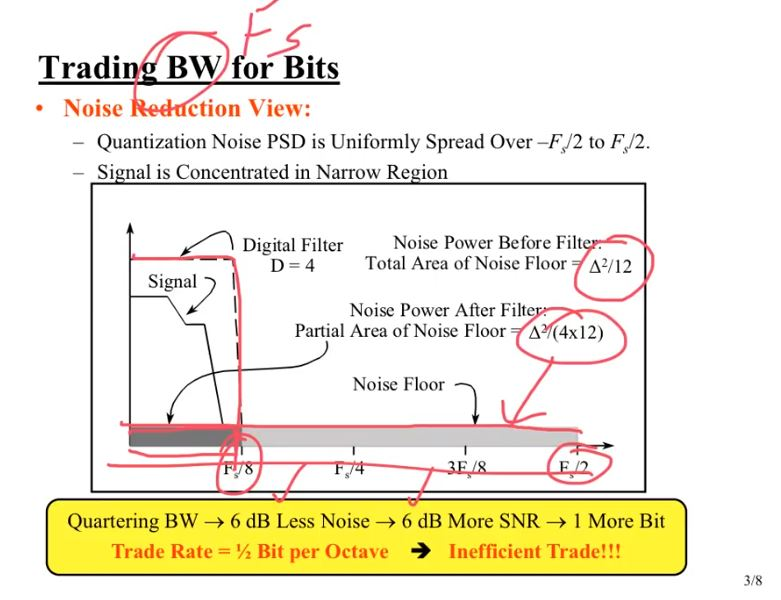
\includegraphics[width = 0.7\textwidth, frame]{Figures/Sampling/oversampling_SNQR_relation}
\caption{Oversampling and SNQR relation}
\label{fig:Sampling:oversampling_SNQR_relation}
\end{figure}	

	\item The noise power is the area under the curve then we divide powers
	
	\end{itemize}

\item So engineers start to search for a better trade-off

\item The idea of $\Sigma-\Delta$ converter: don't touch the signal but push the noise outside the signal spectrum

\newpage
\item Intuition and results are shown in \autoref{fig:Sampling:sigma_delta_noise_shaping}.

	\begin{figure}[h]
\centering
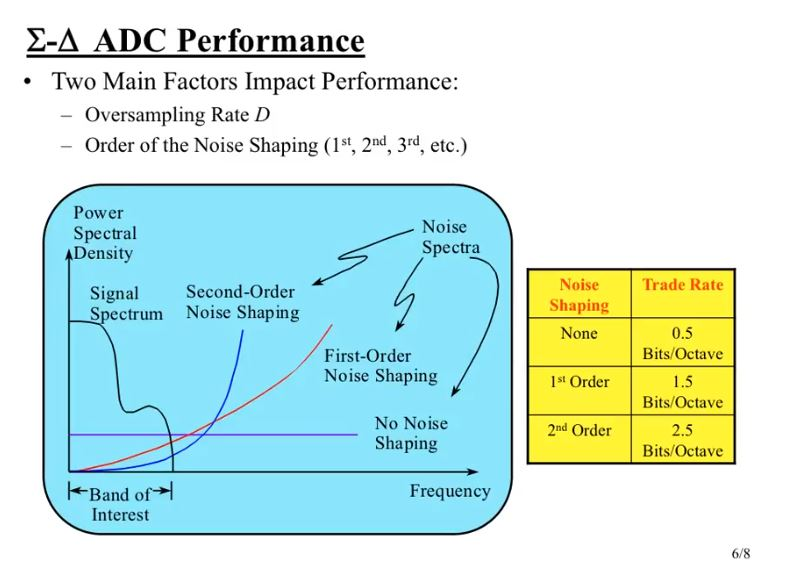
\includegraphics[width = 0.7\textwidth, frame]{Figures/Sampling/sigma_delta_noise_shaping}
\caption{Noise shaping effect}
\label{fig:Sampling:sigma_delta_noise_shaping}
\end{figure}	

	\begin{itemize}
	\item The more we increase the order of noise shaping, the area of the noise decrease and hence SNQR and ENOB increase for the \tbi{band of interest}
	\end{itemize}


\end{itemize}